\chapter{多项式的基础理论}
在初中我们已经学习过多项式及其四则运算,并着重学习了一元多项式的带余除法、余式定理和多元多项式的乘法公式,因式分解。这都是重要的基础知识,在数学和实际中都有广泛的应用,本章将从理论和应用上对多项式的基础知识作进一步的研究、提高,我们研究的重点仍然是一元多项式。

\section{多项式及其代数运算}
多项式的概念我们并不陌生,尤其是一元多项式,每个人都能举出不少例子。它的四则运算也会用各种方法进行。总括我们已经学过的知识,可以一般地系统整理如下:

\subsection{多项式的概念}
\begin{blk}{定义1}
    形如$a_nx^n+a_{n-1}x^{n-1}+\cdots+a_1x +a_0$
的式子,叫做$x$的一元多项式(简称多项式)。其中,$a_i$ $(i=0, 1, 2,\ldots,n)$是已知实数,$n$是已知非负整数。
\end{blk}
.
一元多项式一般简记为$f(x)$或$g(x)$等,即
$$f (x) =a_nx^n+a_{n-1}x^{n-1}+\cdots+a_1x +a_0$$

在多项式$f(x)$中,$a_ix^i$ $(i=0, 1, 2,\ldots,n)$叫做$f(x)$的$i$次项,$a_i$叫做$i$次项的系数;当$a_i\ne 0$时,多项式$f(x)$称为一元$i$次多项式,并把它的次数记作${\rm deg} f(x)=i$。

特别地,当$n=0$时,多项式成为
$f (x) =a$,
这时,若$a_0\ne 0$, 就叫做零次多项式;若$a_0=0$就叫做零多项式,它的次数不定义。

例如,
$f_1(x)=7x^3-1$叫做一元三多项式,$f_2(x)=-5$叫做零次多项式,$f_3(x)=0$叫做零多项式,它不定义次数。

\begin{rmk}
    在初中我们把多项式中的字母。称为未知数,也称为元。现在我们还可以用函数的观点把它称为自变数,甚至可以更一般地称为不定元。它和数作运算时满足数系运算通性,即满足加法和乘法的结合律、交换律以及乘法对加法的分配律;同时,零与1的运算特性、指数运算律仍然适合。
\end{rmk}

这样一来,任何一个$n$次多项式,经过整理合并同类项,总可以写成标准形式
\begin{equation}
f(x)=a_nx^n+a_{n-1}x^{n-1}+\cdots+a_1x +a_0\quad (a_n\ne 0)
\end{equation}
或者
\begin{equation}
    f(x)=a_0+a_1x+\cdots+a_{n-1}x^{n-1}+a_nx^n\quad (a_n\ne 0)
\end{equation}
其中(3.1)称为多项式$f(x)$的降幂标准式,(3.2)称为多项式$f(x)$的升幂标准式。

例如,多项式$g (x) =5x-7x^2+13x^4-8x-x^3+10x^2-1$
经过整理后,可以写成降幂或升幂两种标准形式
\[g (x) =13x^4-x^3+3x^2-3x-1\]
或者
\[g (x) =-1-3x+3x^2-x^3+13x^4\]

\begin{blk}{定义2}
如果用一个已知数$b$去代替多项式中的元$x$, 就得到 
\[f(b)=a_nb^n+a_{n-1}b^{n-1}+\cdots+a_1b +a_0\]
那么,数$f(b)$就叫做当$x=b$时$f(a)$的值。
\end{blk}

\begin{example}
    已知$f(x)=a_3x^3+a_2x^2+a_1x+a_0\quad (a_3\ne 0)$, 试求$f (0)$, $f (1)$, $f (-1)$, $f (m)$。 
\end{example}


\begin{solution}
\[\begin{split}
    f (0) &=a_0\\
    f (1) &=a_3+a_2+a_1+a_0\\
    f (-1) &= -a_3+a_2-a_1+a_0\\
    f (m) &=a_3m^3+a_2m^2+a_1m+a_0
\end{split}\]
\end{solution}

\begin{example}
    已知$f(x)=x^2+2x+8$, 求$f(-x)$, $f(x+1)$。
\end{example}

\begin{analyze}
    由于$-x$, $x+1$都不是已知数,因而所求的$f(-x)$, $f(x+1)$也不会是一个已知数值,严格地说题目已不是求值问题。但我们可以理解为要求用$-x$与$x+1$分别代替$f(x)$中的$x$所得的新多项式。实际上就是换元,其运算程序与求多项式的值是相同的。
\end{analyze}

\begin{solution}
\[\begin{split}
    f(-x)&=(-x)^2+2(-x)+3=x^2-2x+3\\    
    f(x+1)&=(x+1)^2+2(x+1)+3\\
    &=x^2+2x+1+2x+2+3=x^2+4x+6
\end{split}\] 
\end{solution}

\begin{blk}{定义3}
    两个多项式
\[\begin{split}
f (x) &=a_nx^n+a_{n-1}x^{n-1}+\cdots +a_1x+a_0\\
g (x) &=b_nx^n+b_{n-1}x^{n-1}+\cdots+b_1x+b_0.    
\end{split}\]
如果它们的各同次项系数对应相等,即$a_k=b_k$ ($k$为非负整数)我们就说这两个多项式相等,记作$f(x)=g(x)$。
\end{blk}


不难知道,两个非零多项式相等的必要条件是它们的次数相等,即如果$f(x)=g(x)$, 那么${\rm deg}f(x)={\rm deg}g(x)$.

应该指出,如果把多项式看作一个函数式,那么两个多项式相等就可推出当自变数取任意允许值时,两个多项式的值都是相等的。在这种意义下,我们把两个多项式相等也可以说成“恒等”。

\begin{example}
已知多项式
\[f (x) =x^3+ (a+3) x^2+bx-1\]
与多项式
\[g (x) =x^3- (1-b) x^2+ (10-a) x-1\]
相等,试求$a,b$的值。    
\end{example}

\begin{solution}
设$f(x)=g(x)$, 且都已是降幂标准式,所以它们的各同次项系数对应相等。因而有    
\[\begin{cases}
    a+3=-(1-b)\\b=10-a
\end{cases}\Rightarrow\quad
\begin{cases}
    a-b=-4\\ a+b=10
\end{cases}\]
所以
\[a=3,\qquad b=7\]
\end{solution}

\begin{example}
已知一个恒等式:
\[-11x^2+23x=a(3+x)(3-x)+b(2x-1)(3-x)+c(3+x)(2x-1)\]
试求$a,b,c$。
\end{example}

\begin{analyze}
如果设
\[\begin{split}
    f(x)&=-11x^2+23x\\
    g(x)&=a(3+x)(3-x)+b(2x-1)(3-x)+c(3+x)(2x-1)
\end{split}\]
由题目知$f(x)=g(x)$, 再根据定义3, 将$g(x)$的表达式展开并整理成降幂排列的标准式,写出含有$a,b,c$的方程组,
从而解出$a,b,c$; 这样的方法可行,但太繁。还可以从函数的观点出发,由于$f(x)=g(x)$, 所以给$x$代以任意实数$t$, 都有$f(t)=g(t)$。本题中只要恰当选择$x$的值,就可以简便地求出$a,b,c$。
\end{analyze}

\begin{solution}
由已知恒等式右边式子的特点,我们可以分别选取$x=\frac{1}{2},-3, 3$代入,得
\[\begin{cases}
    \frac{35}{4}=\frac{35}{4}a\\
    -168=-42b\\
    -30=-45c
\end{cases}\Rightarrow\quad \begin{cases}
    a=1\\b=4\\c=\frac{2}{3}
\end{cases}\]
\end{solution}

\begin{ex}
\begin{enumerate}
    \item 
    什么叫零次多项式?什么叫零多项式?它们的区别是什么?
    \item 把下列多项式整理成降幂标准式,并分别求出x=1, 10,t时的值
    \begin{enumerate}
        \item $f (2) =\frac{1}{2}x^3-\frac{1}{3}x+\frac{1}{3}x^3-\frac{3}{4}x^2-\frac{1}{2}x-7+\frac{1}{6}x^3$
        \item $g(x)=7+6x+4x^3+5x^2+3x^4+x^6+2x^5$
    \end{enumerate}  
    \item 试求下列等式成立的充要条件
    \begin{enumerate}
        \item $x^2+b_{n+1}x^{n-1}+\cdots+b_1x+b_0=x^n-3x-1$;
        \item $x^2+b_{n+1}x^{n-1}+\cdots+b_1x+b_0=x^m+1$
    \end{enumerate}
\end{enumerate}
\end{ex}

\subsection{多项式的加法与乘法}

关于多项式的加法与乘法,
我们在初中就已经学过。两个多项式进行加法运算的要点是合并同类项,其运算结果叫做这两个多项式的和;两个多项式进行乘法运算的要点是利用分配律和指数运算律,其运算结果叫做这两个多项式的积。

回忆已学过的多项式加法与乘法运算,我们可系统归纳如下:

\subsubsection{加法与乘法的封闭性}

系数在同一个数系范围内的两个多项式$f(x)$与$g(x)$的和$f(x)+g(x)$与积$f(x)g(x)$仍然是一个多项式,而且它们的系数仍在原来数系范围内。这就是多项式加法与乘法的封闭性。

例如,两个有理系数多项式
\[f(x)=2x^3+\frac{1}{2}x^2-x+1,\qquad g(x)=3x^2+2x-3\]
的和与积
\[\begin{split}
    f(x)+g(x)&=2x^3+\frac{7}{2}x^2-5x-2\\
    f(x)g(x)&=6x^5+\frac{11}{2}x^4-26x^3-\frac{25}{2}x^2+23x-3
\end{split}\]
都是有理系数多项式。


\subsubsection{多项式的加法与乘法的基本性质}

对于一元多项式的加法与乘法,有以下性质:
\begin{enumerate}
    \item 满足结合律,即对于任意多项式$f(x),g(x),h(x)$总有
\[\begin{split}
   [ f (x) +g (x) ] +h (x) &=f (x) +[g (x) +h (x) ]\\
    [f (x) \cdot g (x) ] \cdot h (x) &=f (x) \cdot g (x) \cdot [h (x) ]
\end{split}\]    
这就使我们在进行加或乘法的运算中,可以省略括号而按任何顺序进行。

\item 满足交换律,即
\[f (x) +g (x) =g (x) +f(x)\qquad f (x) \cdot g (x) =g (x) \cdot f (x) \]
这就使我们在进行加或乘法的运算中,可以任意交换参加运算的多项式的位置。
\item 满足乘法对加法的分配律,即
\[f (x) \cdot  [g (x) +h (x) ] =f (x) \cdot g (x) +f(x)\cdot h(x)\]
或者 \[[f(x)+g(x)]\cdot h(x) =f(x)\cdot h(z) +g(x)\cdot h(x)\]
\item 存在零多项式。与零次多项式1, 对任意多项式
$f(x)$, 它们满足以下特性:
\[\begin{split}
    0+f (x) &=f (x) +0=f (x) \\
    0\cdot f (x) &=f (x) \cdot 0=0\\
    1\cdot f (x) &=f (x) \cdot 1=f (x) 
\end{split}\].
\item 对于任意多项式
\[f(x)=a_nx^n+a_{n-1}x^{n-1}+\cdots+a_1x+a_0\]
总存在一个多项式$-f(x)$,
\[-f(x)=-a_nx^n+(-a_{n-1})x^{n-1}+\cdots+(-a_1)x+(-a_0)\]
使得$[-f(x)]+f(x)=f(x)+[-f(x)]=0$,我们把这个多项式$-f(x)$称为多项式$f(x)$的负多项式。

例如,多项式$g(x)=\sqrt{2}x^2-x^3$的负多项式就是
\[-g(x)=-\sqrt{2}x^2+x^3\]
\end{enumerate}

\subsubsection{两多项式的和与积的次数}

设$f(x)$是$n$次多项式,$g(x)$是$m$次多项式,那么它们的和$f(x)+g(y)$也是一个多项式,这个多项式的次数$p$有以下几种情形:
\begin{itemize}
    \item 当$m\ne n$时,$p=\max\{m,n\}$
    \item 当$m=n$时,$p\le n$
\end{itemize}

特别地,当$f(x)=-g(x)$时,$f(x)+g(x)$为零多项式,它不定义次数。

两多项式的积$f(x)\cdot g(x)$也是一个多项式,这个多项式的次数$q=m+n$; 特别地,当$f(x)$, $g(x)$之中至少有一为零多项式时,$f(x)\cdot g(x)=0$, 它不定义次数。

\subsubsection{两个多项式的减法}

两多项式的减法运算结果,叫做两多项式的差,记为$f(x)-g(x)$, 其意义为
\[f (x) -g (x) =f (x) + [-g (x) ]\]

由于负多项式$-g(x)$的存在及多项式加法封闭性,因而$f(x)-g(x)$仍是一个多项式,所以多项式对减法也是封闭的。又因为,
\[[f (x) -g (x) ] +g (x) =f (x) \]

所以,多项式的减法是加法的逆运算。

以上各条可知,系数在指定数系范围内的多项式集合,对加、减、乘三种运算都是封闭的,而且对加、乘运算也有着像数系运算通性那样的良好性质,这就大大方便了运算。

对于多元多项式也可以作类似的整理,归纳,这里仅着重指出:
\begin{enumerate}
    \item 多元多项式的每一项的次数,是指所含各个元的指数之和;一个多项式的次数,是指所含各项次数中的最大数。
    \item 如果一个多元多项式的各项次数都相等,那么,这
个多项式就叫做齐次多项式。

例如:$f(x,y)=x^3-2x^2y+3y^3$叫二元三次齐次多项式;$f(x,y,z)=x^2+y^2+z^2-xy-yz-zx$叫做三元二次齐次多项式。

\item 两个齐次多项式的乘积,仍是一个齐次多项式;但
两个齐次多项式的和,却不一定还是齐次多项式。
\end{enumerate}

\begin{ex}
\begin{enumerate}
    \item 已知$f(x)$是$n$次多项式,$g(x)$是$m$次多项式,($m,n$都是非负整数),试问:
    \begin{enumerate}
        \item $f(x),g(x)$分别最多有几项?最少又有几项?
        \item 它们的和$f(x)+g(x)$与积$f(x)\cdot g(x)$最多各有几项?最少各有几项?
    \end{enumerate}
   \item 计算下列各式:
\begin{enumerate}
    \item $(x+a)^4$
    \item $(x+a)(x^3-ax^2+a^2x-a^3)$
    \item $(x-b)(x^n+bx^{n-1}+\cdots+b^{n-1}x+b^n)$
    \item $(x+y+z)^3$
    \item $(x+y+z)(x^2+y^2+z^2-xy-yz-zx)$
\end{enumerate}
   
\item 不求出乘积的所有各项,你能直接写出下列乘积中的$x^3$, $x^5$与$x^8$的系数来吗?
\[(2x^5-3x^4+x^3+2x-7) \cdot (x^4-x^2+x-1)\]
\item 证明:
\begin{enumerate}
\item 若$f(x)\cdot  g(x)=0$, 则$f(x),g(x)$中至少有一个零多项式;
\item 若$(x+p)(x+2q)+(x+2p)(x+q)$是一个多项式的完全平方,则$9p^2-14pq+9q^2=0$。  
\end{enumerate}

\item 若$f(x)=x^n+nx^{n-1}+1$, $g(x)=x^m+mx^{m-1}-1$, 试证明:$f (x) \cdot g (x) =g (x) \cdot f (x)$
\end{enumerate}
\end{ex}

\subsection{多项式的带余除法}

多项式集合对于加、减、乘法都是封闭的,但对于乘法的逆运算——除法却是不封闭的。例如,多项式
$f (x) =1,\; g (x) =x$
就找不出一个多项式$q(x)$, 能使
$f(x) =q(x)\cdot g(x)$。

这个性质与整数集合很相似。正因为这样,在初中我们曾学习了一元多项式的带余除法,并且学习了用长除法,分离系数法,综合除法以及待定系数法去求两个非零多项式的商式和余式。

正和整数的带余除法相似,一元多项式的带余除法,就是由$f(x)$, $g(x)\ne 0$而求出$q(x)$, $r(x)$, 使它们满足
\[f (x) =q (x) \cdot g (x) +r (x) \]
其中,${\rm deg}r(x)<{\rm deg}g(x)$ 或$r(x)=0$。并把
$f(x)$, $g(x)$, $q(x)$和$r(x)$分别称为被除式、除式、商式和余式。


\begin{example}
已知$f(x)=2x^4+x^3+x^2+x+1$, $g(x)=3x^2+2x+3$,试求$f(x)$除以$g(x)$的商式、余式。
\end{example}

\begin{solution}
用分离系数法,作长除法如下: 
\begin{center}
\begin{tikzpicture}
\node at (0,0)[left]{$2+1+1+1+1$};
\node at (0,-1)[left]{$-)\quad 2+\frac{4}{3}+2\qquad\quad\;  $};
\node at (0,-2)[left]{$-\frac{1}{3}-1+1\quad \;\; $};
\node at (0,-3)[left]{$-)\quad  -\frac{1}{3}-\frac{2}{9}-\frac{1}{3}\quad\;\; $};
\node at (0,-4)[left]{$-\frac{7}{9}+\frac{4}{3}+1$};
\node at (0,-5)[left]{$-)\quad -\frac{7}{9}-\frac{14}{27}-\frac{7}{9}$};
\node at (0,-6)[left]{$ +\frac{50}{27}+\frac{16}{9}$};
\node at (0,-6)[right]{……余式};
\draw (-4,-1.5)--(0,-1.5);
\draw (-4,-3.5)--(0,-3.5);
\draw (-4,-5.5)--(0,-5.5);
\draw (0,-1.5)--(0,0.5);
\draw (0,-.5)--(3,-.5);
\node at (0,0)[right]{$3+2+3$};
\node at (0,-1)[right]{$\frac{2}{3}-\frac{1}{9}-\frac{7}{27}$……商式};

\end{tikzpicture}
\end{center}   
因此:\[\begin{split}
    \text{商式}&\quad q(x)=\frac{2}{3}x^2-\frac{1}{9}x-\frac{7}{27}\\
    \text{余式}&\quad r(x)=\frac{50}{27}x+\frac{16}{9}
\end{split}\]
\end{solution}

\begin{example}
    试求$f(x)=4x^4+8x^3-3x^2-7x$除以$g(x)=2x+3$所得的商式$q(x)$,余式$r(x)$。
\end{example}

\begin{solution}
    选用综合除法求解,因为$2x+3=2\left[x-\left(-\frac{3}{2}\right)\right]$,所以用分离系数法作综合除法如下: 
\begin{center}
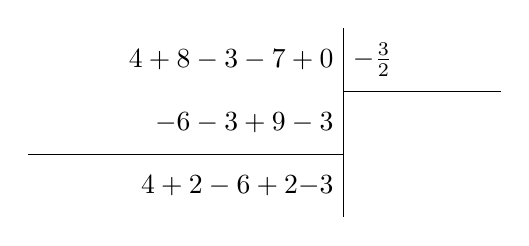
\begin{tikzpicture}[yscale=.8]
\node at (0,0)[left]{$4+8-3-7+0$};
\node at (0,-1)[left]{$-6-3+9-3$};
\node at (0,-2)[left]{$4+2-6+2\boxed{-3}$};
\draw (0,.5)--(0,-2.5);
\draw (0,-.5)--(2,-.5);
\draw (-4,-1.5)--(0,-1.5);
\node at (0,0)[right]{$-\frac{3}{2}$};
\end{tikzpicture}
\end{center}
所以$f(x)$除以$\left(x+\frac{3}{2}\right)$得商式$4x^3+2x^2-6x+2$,余式$-3$。即所求的商式为$q(x)=4x^3+2x^2-6x+2$,余式为$r(x)=-3$。
\end{solution}

容易看出以上两个例子中所得的结果,都符合带余除法恒等式
\[f (x) =q (x) \cdot g (x) +r (x) \]

一般地,多项式带余除法,有以下重要定理:

\begin{blk}{定理}
    对于任意两个多项式$f(x)$, $g(x)\ne 0$, 总是存在唯一的两个多项式$q(x),r(x)$, 使得等式
$f(x) =q(x)\cdot g (x) + r(x) $
成立,并且满足${\rm deg}r(x)<{\rm deg}g(x)$或$r(x)=0$。
\end{blk}

\begin{analyze}
    这个定理的内容既指出了$q(x),r(x)$的存在性——可以找到,又指出了$q(x),r(x)$对于给定的$f(x),g(x)\ne 0$是唯一的——没有第二个。因而,证明理应从这两个方面进行。
\end{analyze}

\begin{proof}
    先证存在性,可按$f(x),g(x)$的次数分为三种情况考虑。
\begin{enumerate}
    \item 若$f(x)=0$, 则不论$g(x)$是什么样的非零多项式,都
可以取$q(x)=r(x)=0$, 显然满足
\[f(x)=q(x)\cdot g(x)+r(x),\quad \text{且}r(x)=0\]
\item 若$f(x)\ne 0$, 且${\rm deg}f(x)<{\rm deg}g(x)$,则可取$q(x)=0$, $r(x)=f(x)$。同样满足
\[f(x)=q(x)\cdot g(x)+r(x),\quad \text{且}{\rm deg}r(x)<{\rm deg}g(x)\]
\item 若$f(x)\ne 0$, 且${\rm deg}f(x)\ge {\rm deg}g(x)$,则可以按下面的方法求出$q(x), r(x)$:

首先用$g(x)$的最高次项去除$f(x)$的最高次项,可得到商$q_1(x)$与余$f_1(x)$,使等式
\begin{equation}
    f (x) =q_1 (x)\cdot y(x)+f_1(x)
\end{equation}
成立,其中$f_1(x)$至少比$f(x)$降低一次,即${\rm deg}f_1(x)<{\rm deg}f(x)$,或$f_1(x)=0$。这时可能有两种情况出现:
\begin{enumerate}
    \item 若${\rm deg}f_1(x)<{\rm deg}g(x)$,或$f_1(x)=0$,我们就取
    \[q(x)=q_1(x),\qquad r(x)=f_1(x)\]
显然定理条件被满足;
\item 若${\rm deg}f_1(x)\ge {\rm deg}g(x)$, 我们就对$f_1(x)$与$g(x)$两个多项式去做上述同样的运算。
\end{enumerate}

其次用$g(x)$的最高次项去除$f_1(x)$的最高次项,可得到商式$q_2(x)$与余式$f_2(x)$, 使等式
\begin{equation}
    f_1(x)=q_2(x)\cdot g(x)+f_2(x)
\end{equation}
成立,其中$f_2(x)$的次数又至少比$f_1(x)$的次数降低一次,即${\rm deg}f_2(x)<{\rm deg}f_1(x)$,或$f_2(x)=0$,这时,
\begin{enumerate}
    \item 若${\rm deg}f_2(x)<{\rm deg}g(x)$,或$f_2(x)=0$,由(3.3)、(3.4)式得
    \[f(x)=[q_1(x)+q_2(x)]\cdot g(x)+f_2(x)\]
    我们就取$q(x)=q_1(x)+q_2(x),\quad r(x)=f_2(x)$。
    定理显然被满足;
    \item 若${\rm deg}f_2(x)\ge {\rm deg}g(x)$,就对$f_2(x)$与$g(x)$做上述同
样运算,同样可以将$f_2(x)$的次数降低至少一次,得到商式$q_3(x)$与余式$f_3(x)$,……作上述同样的分析、处理。
\end{enumerate}

再次,由于${\rm deg}f(x)$是一个非负整数,经过有限次的逐次至少减一,总会有一次(设第$k$次)达到${\rm deg}f_k(x)<{\rm deg}g(x)$或$f_k(x)=0$。于是,我们可得等式
\begin{equation*}
    f_{k-1}(x)=q_k(x)\cdot g(x)+f_k(x) \tag{$k$}
\end{equation*}

综上所述,由等式(3.3)、(3.4)、……($k$),就可以得到
\[\begin{split}
   f(x)&=q_1(x)\cdot g(x)+f_1(x)\\
   &=[g_1(x)+q_2(x)]\cdot g(x)+f_2(x)\\ 
&=\cdots\cdots\\
&=[q_1(x)+q_2(x)+\cdots+q_k(x)]\cdot g(x)+f_k(x)
\end{split}\]
其中,${\rm deg}f_k(x)<{\rm deg}g(x)$或$f_k(x)=0$。

这时,我们就取
\[\begin{split}
    q(x)&=q_1(x)+q_2(x)+\cdots +q_k(x)\\
    r(x)&=f_k(x)
\end{split}\]
显然,这样定理的条件被满足。存在性证毕。
\end{enumerate}

下面再证$q(x)$与$r(x)q$的唯一性。假设除$q(x),r(x)$外,还存在另外一组$q'(x),r'(x)$也满足
\begin{enumerate}
    \item $f(x)=q'(x)\cdot g(x)+r'(x)$,且${\rm deg}r'(x)<{\rm deg}g(x)$或$r'(x)=0$。结合已有的$q(x)$, $r(x)$满足。
    \item $f(x)=q(x)\cdot g(x)+r(x)$,且${\rm deg}r(x)<{\rm deg}g(x)$或$r(x)=0$就可以得出
\[q(x)\cdot g(x)+r(x)=q'(x)\cdot g(x)+r'(x)\]
所以
\[[q(x)-q'(x)]\cdot g(x)=r'(x)-r(x)\]
\end{enumerate}

在此等式中,如果$q(x)-q'(x)\ne 0$,则有
\[{\rm deg}\{[q(x)-q'(x)]\cdot g(x)\}\ge {\rm deg}g(x)\]
但是,由上面的情形又有
${\rm deg}[r'(x)-r(x)]<{\rm deg}g(x)$或$[r'(x)-r(x)]$不定义次数,这是不可能的。所以
\[q'(x)-q(x)=0\quad \Rightarrow\quad q'(x)=q(x)\]

又由于$g(x)\ne 0$,因而$r'(x)-r(x)=0$,即$r'(x)=r(x)$。因此,$q'(x)=q(x)$, $r'(x)=r(x)$。唯一性证毕。
\end{proof}

带余除法是一元多项式的特有运算,但对于二元齐次多项式,我们也可以把其中的一元看作常数来进行带余除法。但是,当余式不为零时,由于选作常数的元的不同,商式与余式也会不同的。

\begin{example}
 已知$f(x,y)=2x^3+7x^2y+13xy^2+5y^3$, $g(x,y)=2x+y$, 试求:
 \begin{enumerate}
     \item 把$y$看作常数时
     \item 把$x$看作常数时
 \end{enumerate}
$f(x,y)$除以$g(x,y)$所得的商式$q(x,y)$与余式$r(x,y)$。
\end{example}

\begin{solution}
\begin{center}
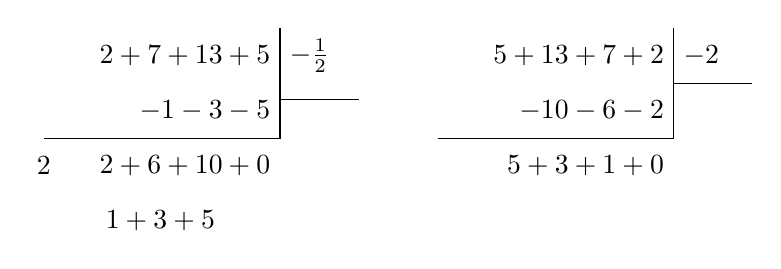
\begin{tikzpicture}[yscale=.7]
\begin{scope}
    \node at (0,0)[left]{$2+7+13+5$};
    \node at (0,-1)[left]{$-1-3-5$};
    \node at (0,-2)[left]{$\boxed{2+6+10}+0$};
    \node at (0,-3)[left]{$1+3+5\qquad $};
    \node at (0,0)[right]{$-\frac{1}{2}$};
    \node at (-3,-2){2};
    \draw (-3,-1.5)--(0,-1.5)--(0,.5);
    \draw (0,-.8)--(1,-.8);
\end{scope}
\begin{scope}[xshift=5cm]
    \node at (0,0)[left]{$5+13+7+2$};
    \node at (0,-1)[left]{$-10-6-2$};
    \node at (0,-2)[left]{$5+3+1+0$};
    \node at (0,0)[right]{$-2$};
    \draw (0,-.5)--(1,-.5);
    \draw (-3,-1.5)--(0,-1.5)--(0,.5);
\end{scope}
\end{tikzpicture}
\end{center}
\begin{enumerate}
    \item $q(x,y)=x^2+3xy+5y^2,\qquad r(x,y)=0$
    \item  $q(x,y)=5y^2+3xy+x^2,\qquad r(x,y)=0$
\end{enumerate}
\end{solution}

\begin{example}
已知$f(x,y)=2x^3+7x^2y+13xy^2+y^3$, $g(x,y)=2x+y$。要求同例3.7。
\end{example}

\begin{solution}
\begin{center}
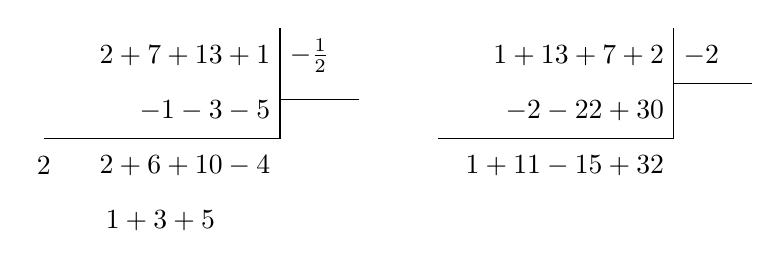
\begin{tikzpicture}[yscale=.7]
\begin{scope}
    \node at (0,0)[left]{$2+7+13+1$};
    \node at (0,-1)[left]{$-1-3-5$};
    \node at (0,-2)[left]{$\boxed{2+6+10}-4$};
    \node at (0,-3)[left]{$1+3+5\qquad $};
    \node at (0,0)[right]{$-\frac{1}{2}$};
    \node at (-3,-2){2};
    \draw (-3,-1.5)--(0,-1.5)--(0,.5);
    \draw (0,-.8)--(1,-.8);
\end{scope}
\begin{scope}[xshift=5cm]
    \node at (0,0)[left]{$1+13+7+2$};
    \node at (0,-1)[left]{$-2-22+30$};
    \node at (0,-2)[left]{$1+11-15+32$};
    \node at (0,0)[right]{$-2$};
    \draw (-3,-1.5)--(0,-1.5)--(0,.5);
    \draw (0,-.5)--(1,-.5);
\end{scope}
\end{tikzpicture}
\end{center}
\begin{enumerate}
    \item $q(x,y)=x^2+3xy+5y^2,\qquad r(x,y)=-4y^3$
    \item  $q(x,y)=y^2+11xy-15x^2,\qquad r(x,y)=32x^3$
\end{enumerate}
\end{solution}

\begin{ex}
\begin{enumerate}
    \item 若$n$次多项式$f(x)$除以$m$次多项式$g(x)$, 试确定所得商式和余式的次数。
    \item 求$f(x)$除以$g(x)$的商式$q(x)$及余式$r(x)$
\begin{enumerate}
    \item $f(x)=x^3+3x^2-x+7,\quad g(x)=x+2$
    \item $f(x)=x^3+3x^2-x+7,\quad g(x)=2x+1$
    \item $f(x)=4x^4+4x^3+5x^2+2x+1,\quad 
g (x) =2x^2+x+1$
    \item $f (x) =x^5+30a^5,\quad g (x) =x+2a$
    \item $f(x)=x^3+3ax^2+(2a^2 -a)x+(a-1),\quad g (x) =x+a-1$
    \item $f(x)=42x^9-13x^7-104x^5+84x^3+9x,\quad 
g (x) =6x^4+11x^2+1$
\end{enumerate}
\item 
若已知除式$g(x)=2x^2-x+3$, 商式$q(x)=x^2-5$, 余式$r(x)=3x+1$, 试求被除式$f(x)$。

\item 试任选一元作常数,求下列$f(x,y)$除以$g(x,y)$所得的商式与余式:
\begin{enumerate}
    \item $f (x,y) =2x^4-x^3y-2x^2y^2-2xy^3-y^4,\quad 
g (x,y) =2x^2+xy+y^2$
    \item $f(x,y)=2x-x^3y-2xy^3-y^4,\quad 
g (x,y) =2x^2+xy+y^2$
\end{enumerate}

\item 求$a^3-b^3+c^3+3abc$除以$a-b+c$所得的商式与余式。
\end{enumerate}
\end{ex}

\section*{习题3.1}
\addcontentsline{toc}{subsection}{习题3.1}
\begin{enumerate}
    \item 试求证
\[\begin{vmatrix}
    a_1+x &  b_1+x  &  c_1+x\\
    a_2+x &  b_2+x  &  c_2+x\\
    a_3+x &  b_3+x  &  c_3+x\\
\end{vmatrix}\]
是一个次数不大于1的多项式或一个零多项式,并求出$p(1)$的值。

\item 不求乘积的各项,只计算下列乘积中$x^{20}$、$x^{12}$两项的系数
\[(a_{13}x^{13}+a_{12}x^{12}+\cdots +a_{1}x+a_0)(b_9x^9+b_8x^8+\cdots +b_1x+b_0)\]
\item 证明恒等式
\[(a^2+b^2)(x^2+y^2)=(ax+by)^2+(bx-ay)^2\]

\item 已知$f(x)=x^7+\frac{1}{128}$, $g(x)=2x+1$,求$f(x)$除以$g(x)$所得的商式$q(x)$及余式$r(x)$。

\item 求$f(x,y)=x^2y+xy^2+xy-x-y-1$除以$g(x,y)=xy-1$所得的商式与余式。
\item 已知
\[\begin{split}
h(x)&=x^2+px+q\\
f(x)&=px^3+(p^2+q)x^2+(2pq+r)x+q^2+s\\
g(x)&=px^3+(p^2-q)x^2+rx-q^2+s
\end{split}\]
试求证:$f(x)$除以$h(x)$, $g(x)$除以$h(x)$分别得到的余式或同时为零,或同时不为零。

\item 如果已知
$f(x)=q(x)\cdot g(x)+r(x)$, 且${\rm deg}r(x)>{\rm deg}g(x)$或$r(x)=0$,$k$是非零常数,试问:
\begin{enumerate}
    \item $kf(x)$除以$g(x)$的商式、余式各是什么?
    \item $f(x)$除以$k\cdot g(x)$商式、余式又是什么?
    \item  $kf(x)$除以$k\cdot g(x)$的商式、余式各是什么?    
\end{enumerate}


\item 已知$f(x)=x^3-2x^2-x+3$, 

试求:$f(-1)$, $f(0)$, $f (x+1) -f (x)$, $f (x^2+1)$。

\item 已知$f(x)=x^4+4x^3+6ax^2+4bx+c$除以$g(x)=x^3+3x^2+9x+3$时的余式$r(x)=0$, 试求$a,b,c$以及商式$q(x)$.

\item 已知$f(x)=x^3+2x^2+3x+2$除以整系数多项式$g(x)$所得的商式和余式都是$h(x)$, 试求$g(x)$与$h(x)$ (其中$h(x)$为非常数的整系数多项式)。
\end{enumerate}

\section{余式定理与因式定理}
在初中代数中已经学习过余式定理,它是直接由带余除法引出来的一个重要定理,在代数学中有一系列的理论和应用价值,本节将进一步学习和推广这一定理。

\subsection{余式定理}

对多项式的讨论,可以从形式上作带余除法,从而求得商式及余式;也可以从函数观 点求得在$x$取某一值时的值,这两种观点有什么联系呢?要沟通这两种观点的方法,就是余式定理。

\begin{blk}{余式定理}
    用一次多项式$x-\alpha$去除多项式$f(x)$所得的余式是一个常数,这个常数就等于$f(\alpha)$。
\end{blk}

\begin{proof}
    $f(x)$除以$x-\alpha$,由带余除法得:
\[f(x)=(x-\alpha)\cdot q(x)+r\]
令$x=\alpha$,即得$f(\alpha)=r$,所以
\[f(x)=q(x)\cdot (x-\alpha)+f(\alpha)\]

这样一来,我们若要求$f(x)$除以一次式$x-\alpha$的余式时,除用带余除法外,还可以用余式定理直接求出多项式的值$f(\alpha)$. 两种观点,两种方法的效果是一样的。
\end{proof}

\begin{example}
    试求$f(x)$除以$g(x)=k(x+\alpha)$所得的余式。
\end{example}

\begin{solution}
除式$g(x)=k\left[x-\left(-\frac{\alpha}{k}\right)\right]$

如果设$g_1(x)=x-\left(-\frac{\alpha}{k}\right)$,则$g(x)=k\cdot g_1(x)$,由余式定理可知$f(x)$除以$g_1(x)$所得的余式为
\[r_1=f\left(-\frac{\alpha}{k}\right)\]
    
又根据习题3.1中第7题的结论:除式乘以一个非零数$k$时,余式不变,所以$f(x)$除以$g(x)$所得的余式就等于$f(x)$除以$g_1(x)$所得的余式。所以
\[r=r_1=f\left(-\frac{\alpha}{k}\right)\]
\end{solution}


\begin{example}
    试求$f(x)$除以$g(x)=(x-\alpha)(x-\beta)$的余式。
\end{example}

\begin{solution}
设$f(x)$除以$g(x)$所得的商式为$q(x)$,余式为$r(x)$,则有
\begin{equation}
f(x)=q(x)(x-\alpha)(x-\beta)+r(x)
\end{equation}
    其中,$0\le {\rm deg}r(x)<2$或$r(x)=0$。

因而可进一步设$r(x)=ax+b$,代入(3.5)得
\begin{equation}
    f(x)=q(x)(x-\alpha)(x-\beta)+ax+b
\end{equation}
令$x=\alpha$,由(3.6)得
\begin{equation}
    f(\alpha)=a\alpha+b
\end{equation}
令$x=\beta$,由(3.6)得
\begin{equation}
    f(\alpha)=a\beta+b
\end{equation}
将(3.7), (3.8)联立可以解出
\[a=\frac{f(\alpha)-f(\beta)}{\alpha-\beta},\qquad b=\frac{\alpha f(\beta)-\beta f(\alpha)}{\alpha-\beta}\]
所以,所求的余式为
\[r(x)=\frac{f(\alpha)-f(\beta)}{\alpha-\beta}x+\frac{\alpha f(\beta)-\beta f(\alpha)}{\alpha-\beta}\]
\end{solution}

\begin{ex}
\begin{enumerate}
\item 设$f(x)=x^5-6x^3+x^2-20x+24$, 试求$f(x)$除以下列各式的余数:
\[x-1;\qquad  x+1;\qquad  2x+1;\qquad  3x-2\]
\item 试求
\begin{enumerate}
\item $k\cdot f(x)$除以$x-\alpha$的余式;
\item $(x^2+1)f(x)$除以$x+\beta$的余式;
\item $k(x^2-1)f(x)+3x-1$除以$x-m$的余式。
\end{enumerate}

\item 如果$f(x)$除以$-2$的余式为2, 除以$x+3$的余式为
4, 那么$f(x)$除以$x^2+x-6$的余式是什么?
\end{enumerate}
\end{ex}



\subsection{因式定理}

两个多项式做带余除法时,如果$f(x)$除
以$g(x)$所得的余式$r(x)=0$, 即
\[f (x) =q (x) \cdot g (x) \]
我们就说$f(x)$能被$g(x)$整除,也可以说$g(x)$整除$f(x)$或$g(x)$是$f(x)$的一个因式,$f(x)$是$g(x)$一个倍式。显然,它们的商式$q(x)$也是$f(x)$的一个因式,而$f(x)$也是$q(x)$的一个倍式。

由余式定理可以推证出下列因式定理:

\begin{blk}{因式定理}
$(x-\alpha)$是$f(x)$的一个因式的必要充分条件是$f (\alpha) =0$。
\end{blk}

\begin{proof}
  先证必要性。由于$(x-\alpha)$是$f(x)$的一个因式,因而有
\[f (x) = (x-\alpha ) \cdot q (x) \]
这就是说,$f(x)$除以$x-\alpha$ 时,余式$r=0$.

但由余式定理知,$f(x)$除以$x-\alpha$ 的余式为$f(\alpha )$, 因此,
$f (\alpha) =0$。

再证充分性。由于$f(\alpha )=0$, 因而根据余式定理可以得出
\[f (x) =q (x) \cdot  (x-\alpha ) +f (\alpha ) \]
即
\[f (x) =q (x) (x-\alpha )\]
因此$x-\alpha$ 是$f(x)$的因式。  
\end{proof}


我们已经知道,若在$x=\alpha$ 时,$f(x)$的值$f(\alpha )=0$, 则称$\alpha$ 是$f(x)$的一个根,或者说,$\alpha$是$f(x)$的一个零点。如,
$f(x)=2x^2-7x+3$, 由于$f\left(\frac{1}{2}\right)=f(3)=0$, 因而就说$\frac{1}{2}$,
3都是$f(x)$的根。

这样一来,因式定理又可以叙述为:$(x-\alpha)$是$f(x)$的一个因式的充要条件是$\alpha$ 为$f(x)$的一个
根。

因式定理还可以推广到一般,这就是:

若$(x-\alpha_1)(x-\alpha_2)\cdots(x-\alpha_k)$是$f(x)$的因式的必要充分条件是$f(\alpha_1)=f(\alpha_2) =\cdots=f(\alpha_k)=0$. 也就是$\alpha_1,\alpha_2,\ldots,\alpha_k$都是$f(x)$的根(其中$\alpha_1,\alpha_2,\ldots,\alpha_k$两两不等)。

\begin{proof}
必要性是显然的,因为若对于两两不等的数$\alpha_1,\alpha_2,\ldots,\alpha_k$来说,$(x-\alpha_1)(x-\alpha_2)\cdots(x-\alpha_k)$都是$f(x)$的因式,
则有    
\[f(x)=(x-\alpha_1)(x-\alpha_2)\cdots(x-\alpha_k)\cdot q(x)\]
所以$f(\alpha_1)=f(\alpha_2) =\cdots=f(\alpha_k)=0$

即$\alpha_1,\alpha_2,\ldots,\alpha_k$为$f(x)$的$k$个不同的根。

再证充分性,由于$f(\alpha_1)=0$, 因而根据因式定理可
有
\begin{equation}
    f (x) = (x-\alpha_1) \cdot q_1 (x)
\end{equation}

将$x=\alpha_2$代入上式,得
\[f (\alpha_2) = (\alpha_2-\alpha_1) \cdot q_1(\alpha_2)\]
其中,因$f(\alpha_2)=0$, $\alpha_2-\alpha_1\ne 0$, 所以
\[q_1(\alpha_2)=0\]
再根据因式定理,就得出$\alpha_2$是$g_1(x)$的根,即
\begin{equation}
q_1(x)=(a-\alpha_2)\cdot q_2(x)
\end{equation}
将(3.10)代入(3.9)得
\begin{equation}
    f (x) = (x-\alpha_1) (x-\alpha_2)\cdot q_2(x)
\end{equation}
就这样逐步推下去,我们可以得到
\begin{equation}
    f (x) = (x-\alpha_1 ) (x-\alpha_2)\cdots(x-\alpha_{k-1})\cdot q_{k-1}(x) 
\end{equation}
将$x=\alpha_k$代入(3.11)式,得
\[f (\alpha_k) = (\alpha_k -\alpha_1)\cdots (\alpha_k-\alpha_{k-1})\cdot q_{k-1}(\alpha_k)\]
其中,已知$f(\alpha_k)=0$, 且$(\alpha_k-\alpha_1),(\alpha_{k}-\alpha_2),\ldots,(\alpha_k-\alpha_{k-1})$都不等于零,因而有 $q_{k-1}(\alpha_k)=0$。

由因式定理可知$\alpha_k$为$q_{k-1}(x)$的一个根,即
\begin{equation}
    q_{k-1}(x)=(x-\alpha_k)\cdot q_{k}(x)
\end{equation}
将(3.13)式代入(3.12)式,就得出所证结论:
\[f(x)=(x-\alpha_1)(x-\alpha_2)\cdots(x-\alpha_{k-1})(x-\alpha_k)\cdot q_k(x)\]
即:$(x-\alpha_1),(x-\alpha_2),\ldots,(x-\alpha_k)$都是$f(x)$的因式。
\end{proof}

因式定理及推广在沟通两种观点研究多项式的问题上,作用更为突出。数$\alpha$是多项式的一个零点(根)、一次式$(x-\alpha)$是$f(x)$的一个因式、一次式$(x-\alpha)$能够整除$f(x)$、$f(\alpha)=0$都是同一件事情的不同说法,在多项式理论的学习中是很重要的。


\begin{example}
证明恒等式
\[a^2(b-c)+b^2(c-a)+c^2(a-b)=(a-b)(b-c)(c-a)\]
\end{example}

\begin{proof}
等式左边是一个三元多项式,可以分别将$a,b,c$看作元,同时将$b,c$; $a,c$; $b,a$看作常数,依次将$a=b$, $b=c$, $c=a$代入,分别得到
\[\begin{split}
   b^2 (b-c) +b^2 (c-b) +c^2 (b-b) =0\\
   a^2 (c-c) +c^2 (c-a) +c^2 (a-b) =0\\
a^2(b-a)= b^2(a-a) + a^2(a-b) =0 
\end{split}\]

因此,根据因式定理可得
\[a^2 (b-c) +b^2 (c-a) +c^2 (a-b)=k (a-b) (b-c)(c-a)\]
由多项式恒等不难断定$k=1$. 所以
\[a^2 (b-c) +b^2 (c-a) +c^2 (a-b)
= (a-b) (b-c)(c-a)\]
\end{proof}

\begin{example}
    已知$f(x)=x^3+px^2+qx+6$含有因式$(x-3)(x-1)$, 试求$p,q$的值及$f(x)$的另一个一次因式。
\end{example}

\begin{solution}
    由已知可设$f(x)$的另一个一次因式为$ax+b$,因此:
\[f(x)=x^3+px^2+qx+6=(x-3)(x-1)(ax+b)\]
即:
\[x^3+px^2+qx+6=ax^3+(-4a+b)x^2+(3a-4b)x+3b\]
由待定系数法,可以求出
\[a=1,\qquad b=2,\qquad p=-2,\qquad q=-5\]
所以,$f(x)$的另一个一次因式为$x+2$。
\end{solution}

\begin{ex}
\begin{enumerate}
    \item 用因式定理分解因式
\begin{multicols}{2}
\begin{enumerate}
    \item $x^3-3x+2$
    \item $2x^3-x^2-5x-2$
\end{enumerate}
\end{multicols}
    \item 已知$f(x)=3x^3+mx^2+nx-2$含有因式$3x-2$,且$f(-1)=-20$,试求$m,n$的值。
    \item 试证明恒等式
\[a^2(b+c)+b^2(c+a)+c^2(a+b)+2abc=(a+b)(b+c)(c+a)\]
\end{enumerate}  
\end{ex}

\subsection{余式定理、因式定理的推论}

在余式定理与因式定理的基础上,对一元多项式,还有下面两个重要推论:

\begin{blk}{推论1}
    一元$n$次多项式$f(x)$最多只能有$n$个不相同的根。
\end{blk}

\begin{proof}
设$f(x)=a_nx^n+a_{n-1}x^{n-1}+\cdots+a_1x+a_0\quad (a_n\ne 0)$,若已知两两不等的$n$个数
$\alpha_1, \alpha_2, \ldots, \alpha_n$
都是$f(x)$的根,则由因式定理可知
\begin{equation}
    f (x) = (x-\alpha_1) (x-\alpha_2)\cdots (x-\alpha_n)\cdot q(x)
\end{equation}
但由于${\rm deg}f(x)=n$, 且${\rm deg}[(x-\alpha_1)(x-\alpha_2)\cdots(x-\alpha_n)]=n$, 所以(3.14)式中$q(x)$只能是零次多项式,即${\rm deg}g(x)=0$, 再由多项式相等的定义,可知
\[q (x) =a_n\ne 0\]

若再选任一个与$\alpha_i,\; (i=1, 2,\ldots,n)$都不相等的数$\alpha_{n+1}$代入(3.14)式,得
\[f(\alpha_{n+1})=(\alpha_{n+1}-\alpha_{1})(\alpha_{n+1}-\alpha_2)\cdots (\alpha_{n+1}-\alpha_n)\cdot \alpha_n\]
其中,由$\alpha_i,\; (i=1, 2,\ldots,n,n+1)$都不相等,可知
\[\alpha_{n+1}-\alpha_i\ne 0\;  (i=1, 2,\ldots,n),\quad \text{且}\quad a_n\ne 0\]
$\therefore\quad f(\alpha_{n+1}) \ne 0$

因此,$\alpha_{n+1}$不是$f(x)$的根,所以,$f(x)$最多只有$n$个不同根。
\end{proof}

\begin{blk}{推论2}
如果多项式$f(x)$与$g(x)$的次数都不大于$n$, 且有$n+1$个两两不相等的数$\alpha1,\alpha2,\ldots,a_{n+1}$能使这两个多项式相应的值相等,即   
\[f(\alpha_i)=g(\alpha_i)\quad (i=1,2,\ldots,n,n+1)\]
 那么,这两个多项式必定相等,即$f(x)=g(x)$。
\end{blk}

\begin{proof}用反证法。
假设,$f(x)\ne g(x)$, 则多项式
$F (x) =f (x) -g (x)$
就是一个次数不大于$n$的多项式。但是由已知条件知道
\[F (\alpha_i) =f (\alpha_i) -g (\alpha_i)=0,\quad  (i=1,2,\ldots,n,n+1)\]
这就是说,$F(x)$有$n+1$个不同的根。这与推论1的结论是矛盾的。所以
$f (x) =g (x)$。
\end{proof}

\begin{example}
    不用乘法展开下式,求证:
\[x(x-1) (x-2)(x-3)+1=(x^2-3x+1)^2\]
\end{example}

\begin{proof}
    设$f(x)=x(x-1)(x-2)(x-3)+1$, $
g (x) = (x^2-3x+1)^2$。
由于它们都是4次多项式,因而根据推论2,只要验证当$x$取任    
意五个不同的数时,这两个多项式对应的值都相等就可以了,

分别取$x=0, 1, 2, 3, 4$, 则可得:
\[f (0) =1=g (0);\qquad f (1) =1=g (1) ;\qquad f (2) =1=g (2)\]
\[ f (3) =1=g (3) ;\qquad f (4) =25=g (4) \]
所以$f (x) =g (x) $,即:
\[x (x-1) (x-2) (x-3)+1=(x^2-3x+1)^2\]
\end{proof}


\begin{example}
已知$f(x)$是一个五次多项式,且可被$x^2-2$整除,且$f(1)=f(-1)=0$, 试确定这个多项式$f(x)$的各项系数间的关系。
\end{example}

\begin{solution}
设 $f(x)=ax^5+bx^4+cx^3+dx^2+ex+f$,由已知及因式定理可知
\[f (x) = (x^2-2) (x+1)(x-1)\cdot q(x)\]
又由于$f(x)$是五次多项式,因而$q(x)$必定是一次式,不妨设为:$q(x)=mx+n\; (m\ne 0)$。所以
\[ax^5+bx^4+cx^3+dx^2+ex+f= (x^2-2) (x+1)(x-1)(mx+n)\] 
即
\[ax^5+bx^4+cx^3+dx^2+ex+f= mx^5+nx^4-3mx^3-3nx^2+2mx+2n\] 

由多项式相等的定义可得:
\[\begin{cases}
    a=m\\
    b=n\\
    c=-3m\\
    d=-3n\\
    e=2m\\
    f=2n
\end{cases}\qquad (m\ne 0)\]

由此方程组可消去$m,n$,就得
\[\begin{cases}
    a=-\frac{1}{3}x=\frac{1}{2}e\ne 0\\
    b=-\frac{1}{3}d=\frac{1}{2}f
\end{cases}\Rightarrow\quad \begin{cases}
    6a=-2c=3e\ne 0\\
    6b=-2d=3f
\end{cases}\]
这就是$f(x)$的各系数之间的关系。
\end{solution}

\begin{ex}
\begin{enumerate}
    \item 已知$f(1)=f(3)=0$, $f(2)=-4$, 试求二次多项式$f (x)$。
    \item 已知$f(-1)=f(-4)=2$, $f(-3)=8$, $f(-2)=4$。试求三次多项式$f(x)$。
    \item 一个三次多项式$f(x)$, 已知$f(x)+1$可被$(x+1)^2$整除;又$3-f(x)$有一个根为$-2$, 并含有一个因式为一次二项式的平方。试求$f(x)$。
\end{enumerate}
\end{ex}

\section*{习题 3.2}
\addcontentsline{toc}{subsection}{习题 3.2}
\begin{enumerate}
    \item 
已知$f(x)=x^3+3x^2+x+1$, 求$f(x-1)$, $f(x+1)$, $f (-x^2)$
\item 已知$f(x-1)=x^3+3x^2+x-1$, 求$f(x)$, $f(-x)$。
\item 已知$f(x)=x^3+ax^2+5x-4$, 且$f(2)=f(-3)$, 试求$a$及$f(2)$。
\item 若有一多项式$g(x)$, 已知$g(-1)=1$, $g(4)=11$, 试求$f(x)$被$(x+1)(x-4)$除后的余数。

\item 如果$f(x)$被$2x-3$除以后余数为4, 试求多项式
$(x^2+1)\cdot f(x)+7$被$2x-3$除的余数。
\item 已知恒等式
\[x^3+x^2+x+1=a+b (x+1) +c (x+1) (x+3)+d (x+1) (x+3)(x+5)\]
试求$a,b,c,d$的值。
\item 用余式定理及其推论证明:
\[\begin{split}
   & (b-c) (x-b)(x-c)+(c-a)(x-c)(x-a)\\
&\qquad + (a-b) (x-a)(z-b)+(a-b)(b - c)(c-a)=0
\end{split}\]
\item 证明$2b^2c^2+2c^2a^2+2a^2b^2-a^4-b^4-c^4$ 能被$(a+b+c)(b+c-a)(c+a-b)(a+b-c)$整除,
并求其商式。
\item 若$f(x)=x^3+kx^2-20x+6$ 能被$x-3$整除,试求常
数$k$。
\item 若$f(x)=2x^3-x^2+ax+b$能被$(x+2)(x-4)$整除,
试求常数$a,b$。
\item $f(x)=2x^3-ax+1$, $g(x)=x^3+5x+b$ 能不能有四个不同的数$\alpha_1,\alpha_2,\alpha_3,\alpha4$, 使得$f (\alpha_i) =g (\alpha_i)\quad  (i=1,2,3,4)$,
为什么?
\item 利用因式定理,分解因式
\begin{enumerate}
    \item $x^3-3x+2$
    \item $x^3-(a+2b)x^2+b(2a+b)x-ab^2$
\end{enumerate}

\item 如果$x^2+5xy+ay^2+x-y-2=f(x,y)$可以分解为$x,y$的一次因式的积,试求$a$的值。
\end{enumerate}

\section{最高公因式与辗转相除法}
关于两个多项式的公因式、最高公因式的概念,我们在初中代数中已经学过,同时,我们还学习过用辗转相除、分解因式两种方法去求最高公因式,还学习了两个多项式的公倍式与最低公倍式以及求最低公倍式的方法,并得出了最低,公倍式与最高公因式之间的关系
\[[f(x),g(x)]=\frac{k\cdot f(x)\cdot g(x)}{(f(x)\cdot g(x))}\]

由于最高公因式与辗转相除法在多项式理论中占有重要地位,本节将重点进一步加深学习这两个内容。

\subsection{最高公因式}

首先,我们在已经学习的基础上,较严格地给出最高公因式的定义:

\begin{blk}{定义}
 对给定的非零多项式$f(x),g(x)$, 如果有一个多项式$d(x)$, 能满足以下三个条件:   
\begin{enumerate}
    \item $d(x)$的首项系数为1,
    \item $d(x)$是$f(x)$与$g(x)$的公因式,
    \item $d(x)$是$f(x)$与$g(x)$的其它任何一个公因式$\ell(x)$
    的倍式,即$f(x)$与$g(x)$的任一公因式$\ell(x)$是$d(x)$的因式。那么,$d(x)$就叫做多项式$f(x)$与$g(x)$的最高公因式,一般记作
    $(f (x) ,g (x) ) =d (x)$
\end{enumerate}
\end{blk}

上述的条件1是为了保证$(f(x),g(x))$的唯一性而提出的。事实上,若$d(x)$, $d_1(x)$都是$f(x)$与$g(x)$的最高公因式,则由条件2、3就可得出$d(x)$与$d_1(x)$能互相整除,这就有$d(x)=kd_1(x)$, 再由条件1就得到$d(x)=d_1(x)$. 这
就说明,$(f(x),g(x))$如果存在,一定是唯一的。

我们还知道,若$f(x),g(x)$都已分解成不可约的因式的乘积,则在$f(x),g(x)$的所有公因式中,取每一个公因式的指数较小者,这些因式的乘幂的乘积,再乘以一个能使其首项系数为1的常数,就是$(f(x),g(x))$。这就是我们常用的求最高公因式的视察法。


\begin{example}
$f(x)=x(2x-1)^4(x+3)^3$,$g(x)=x^2(2x-1)^2(x+2)^2$

试求$(f(x),g(x))$
\end{example}

\begin{solution}
    公因式为$x,2x-1$,$x$的指数$f(x)$中的1,$2x-1$的指数取$g(x)$中的2,得:
\[(f(x),g(x))=k\cdot x (2x-1)^2\]
$k$是待定系数,为使$(f(x),g(x))$的首期系数为1,显然应取$k=\frac{1}{4}$,所以
\[(f(x),g(x))=\frac{1}{4}  x (2x-1)^2\]
\end{solution}

\begin{example}
$f(x)=x^2-3x+2$, $g(x)=x^4-3x^3+5x^2-8x+5$

试求$(f(x),g(x))$
\end{example}

\begin{solution}
由视察知,$f(x)=(x-1)(x-2)$,因而$(f(x),g(x))$不可能有$(x-1)$, $(x-2)$外的因式,再由因式定理,求得$g(1)=0,\; g(2)\ne 0$,所以$x-1$是$f(x), g(x)$唯一的公因式。所以
\[(f(x),g(x))=x-1\]
\end{solution}

\begin{blk}{定理1}
    给定非零多项式$f(x),g(x)$, 对于任意两个多项式$u(x),v(x)$来说,$f(x),g(x)$的公因式也一定是
$u(x)\cdot f(x)+v(x)\cdot g(x)$的因式。
\end{blk}

\begin{proof}
  设$d(x)$是$f(x)$与$g(x)$的一个公因式,则
\[f (x) =d (x) \cdot f_1 (x),\qquad  g(x)=d(x)\cdot g_1(x)\]
所以
\[u (x) \cdot f (x) +v (x) \cdot g (x) =d (x) [u (x) \cdot f_1 (x) +v (x) \cdot g_1 (x) ]\]
即$d(x)$也是$u(x)\cdot f(x)+v(x)\cdot g(x)$的一个因式。  
\end{proof}

\begin{example}
已知$f(x)=x^4-x^3+3x^2-4x-12$, $g(x)=x^4-x^3+2x^2+3x-22$。

求$(f(x),g(x))$。
\end{example}

\begin{analyze}
应用定理1的结论,我们可以取$u(x)=1$, $v(x)=-1$,从而可得 $f(x)-g(x)=x^2-7x+10$. 只要从 $x^2-7x+10$的因式中就可以找出$f(x),g(x)$的公因式的范围,再应用因式定理即可确定$(f(x),g(x))$。
\end{analyze}

\begin{solution}
因为$f(x)-g(x)=x^2-7x+10=(x-2)(x-5)$,所以$f(x),g(x)$的一次公因式只可能是$x-2$与$x-5$,于是由因式定理,求得
$f(2)=g(2)=0$,但$f(5)\ne 0$。所以$(f(x),g(x))=x-2$。
\end{solution}

\begin{example}
    已知$f(x)=2x^3-3x^2-3x+2$, $g(x)=3x^3-2x^2-7x-2$。求$(f(x),g(x))$。
\end{example}

\begin{solution}
    因为$f(x)+g(x)=5x^3-5x^2-10x=5x(x+1)(x-2)$其中$x$显然不是$f(x),g(x)$的公因式,再用综合除法求得
\[x+1|f(x),\qquad x+1|g(x),\qquad x-2|f(x),\qquad x-2|g(x)\]
所以
\[(f(x),g(x))=(x+1)(x-2)\]
\end{solution}

\begin{ex}
    求下列各组多项式的最高公因式:
\begin{enumerate}
    \item $f(x)=\poly{1,0,0,-1},\quad g(x)=\poly{1,2,3,2,1}$
    \item $f(x)=2x^3-3x^2-11x+6,\quad g(x)=\poly{4,3,-9,2}$
    \item $f(x)=\poly{2,-5,0,-2,1},\quad g(x)=\poly{2,-7,6,-4,1}$
\end{enumerate}
\end{ex}

\subsection{辗转相除法}

辗转相除法的理论基础在于多项式的带余除法及本节的定理1.

\begin{blk}{定理2}
    对于非零多项式$f(x)$, $g(x)$, $r(x)$, 若存在多项式$q(x)$使得$f(x)=q(x)\cdot g(x)+r(x)$, 则有
    \[\big(f(x),\; g(x)\big)=\big(g(x),\; r(x)\big)\]
\end{blk}

\begin{proof}
设$\big(g(x),\; r(x)\big)=d(x)$,则
\begin{enumerate}
\item $d(x)$首项系数是1;
\item $d(x)$是$g(x)$, $r(x)$的公因式,由定理1可知,
$d(x)$也是$f(x)$的因式,因而也是$f(x),g(x)$的公因式;    
\item 再设$f(x)$, $g(x)$的任一个公因式为$\ell(x)$, 由于$r(x)=f(x)-q(x)\cdot g(x)$, 所以,$\ell(x)$也是$r(x)$的一个因式,因而$\ell(x)$就是$g(x),r(x)$的公因式,再由最高公因式的定义知,$\ell(x)$是$d(x)$的因式。所以
\[\big(f (x) ,g (x) \big) =d (x) = \big(g (x) ,r (x) \big)\]
\end{enumerate}
\end{proof}

这样一个定理对于求两个已知多项式的最高公因式起到一些什么作用呢?两个多项式中总有一个多项式的次数不大于另一个多项式的次数,不妨设$g(x)$设的次数不大于$f(x)$的次数,则因在带余除法中,$r(x)$的次数小于$g(x)$的次数或$r(x)=0$. (注意,定理2并不要求$r(x)$满足带余除法中对余式的要求,但带余除法中的余式满足定理2中$r(x)$的条件)这就说明$r(x)$的次数小于$f(x)$的次数,把求$\big(f(x), g(x)\big)$转化为求$\big(g(x), r(x)\big)$实际上是一个降次的过程。

次数是降低了,那么有没有把握求出$\big(g(x),r(x)\big)$呢?
现在可以对$g(x)$, $r(x)$再进行带余除法,求出又一个余
式$r_2(x)$(为了易于辨别,我们把第一次余式记为$r_1(x)$,类似地把第一次第二次所得的商式分别记为$q_1(x)$, $q_2(x)$, 以后以此类推),循此以往,可得到一系列的带余除法:
\begin{equation}
    \begin{split}
f(x)&=q_1(x)g(x)+r_1(x),\quad {\rm deg}r_1(x)<{\rm deg}g(x)\\
g(x)&=q_2(x)r_1(x)+r_2(x),\quad {\rm deg}r_2(x)<{\rm deg}r_1(x)\\
r_1(x)&=q_3(x)r_2(x)+r_3(x),\quad {\rm deg}r_3(x)<{\rm deg}r_2(x)\\
r_2(x)&=q_4(x)r_3(x)+r_4(x),\quad {\rm deg}r_4(x)<{\rm deg}r_3(x)\\
\cdots &\cdots \cdots \cdots \\
r_{i-1}(x)&=q_{i+1}(x)r_i(x)+r_{i+1}(x),\quad {\rm deg}r_{i+1}(x)<{\rm deg}r_i(x)\\
\cdots &\cdots \cdots \cdots \\
r_{s-1}(x)&=q_{s+1}(x)r_s(x)
\end{split}
\end{equation}

最后一个等式表示$r_s(x)$整除$r_{s-1}(x)$, 或者说$r_{s+1}(x)=0$。此时就有
\[\begin{split}
    \big(f(x), g(x)\big)&=\big(g(x),r_1(x)\big)=\big(r_1(x),r_2(x)\big)=\cdots\\
    &=\big(r_i(x),r_{i+1}(x)\big)=\cdots\\
    &=\big(r_{s-1}(x),r_s(x)\big)
\end{split}\]

显然有$\big(r_{s-1}(x),r_s(x)\big)=\frac{1}{c}r_s(x)$,其中:$c$是$r_s(x)$首项系
数。因此:
\[\big(f(x), g(x)\big)=\frac{1}{c}r_s(x)\]

自然会提出这样一个问题,如果始终不能整除,怎么办?我们来证明不会出现始终不能整除的情况。

设${\rm deg}g(x)$是一个有限的非负整数$m$。若$r_1(x)\ne 0$, 令${\rm deg}r_i(x)=m_i$,则
\[m>m_1>m_2>\cdots>m_i>\cdots>m_{s-1}>m_s\]
注意到$m$和所有$m_i$都是非负整数,而数列$m,m_1,m_2,\ldots,m_i,\ldots$
是一个严格递减的数列,则这个数列一定是有限的。例如$m=100$时,数列最多不会超过101项。在某种情形下,若$m_s=0$, 即$r_s(x)$是一个非零常数时,$r_s(x)$就整除$r_{s-1}(x)$了。在这种情况下,$\big(f(x),g(x)\big)=1$, 我们说$f(x)$与$g(x)$互质。这就说明,即使$f(x)$, $g(x)$互质,它们的最高公因式1仍可由上述累次的带余除法求得,由此我们得到:

\begin{blk}{定理3(辗转相除法定理)}
  任给两个非零多项式$f(x)$, $g(x)$进行(3.15)式所给出的辗转相除,通过有限次的运算总可求出唯一存在的$\big(f(x),g(x)\big)$。
\end{blk}

 存在性已在前面叙述,至于唯一性则在给出$\big(f(x),g(x)\big)$的定义后即已阐明。  

\begin{example}
$f(x)=\poly{6,-4,-11,-3,-3,-1}$, 

$g(x)=\poly{4,2,-18,3,-5}$

求$\big(f(x),g(x)\big)$
\end{example}

\begin{solution}
\begin{center}
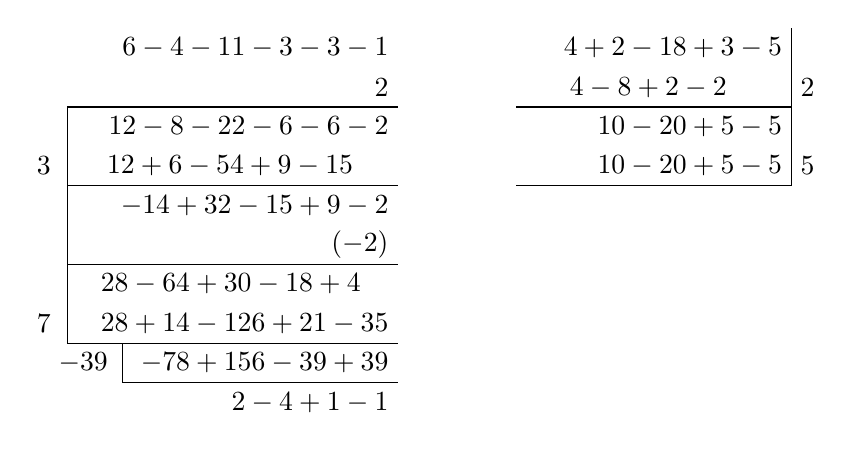
\begin{tikzpicture}
\begin{scope}
\node at (0,0)[left]{$6-4-11-3-3-1$};
\node at (0,-0.5)[left]{$\x 2$};
\node at (0,-1)[left]{$12-8-22-6-6-2$};
\node at (0,-1.5)[left]{$12+6-54+9-15\quad\;$};
\node at (0,-2)[left]{$-14+32-15+9-2$};
\node at (0,-2.5)[left]{$\x(-2)$};
\node at (0,-3)[left]{$28-64+30-18+4\quad$};
\node at (0,-3.5)[left]{$28+14-126+21-35$};
\node at (0,-4)[left]{$-78+156-39+39$};
\node at (0,-4.5)[left]{$2-4+1-1$};

\foreach \x in {-.75, -1.75, -2.75, -3.75}
{
    \draw (-4.2,\x)--(0,\x);
}
\draw (-3.5,-4.25+.5)--(-3.5,-4.25)--(0,-4.25);
\draw (-4.2,-.75)--(-4.2,-3.75);
\node at (-4.5,-1.5){3};
\node at (-4.5,-3.5){7};
\node at (-4,-4){$-39$};
\end{scope}
\begin{scope}[xshift=5cm]
    \node at (0,0)[left]{$4+2-18+3-5$};
\node at (0,-0.5)[left]{$4-8+2-2\qquad $};
\node at (0,-1)[left]{$10-20+5-5$};
\node at (0,-1.5)[left]{$10-20+5-5$};
\foreach \x in {-.75, -1.75}
{
    \draw (-3.5,\x)--(0,\x);
}
\draw (0,-1.75)--(0,.25);
\node at (.2,-.5){2};
\node at (.2,-1.5){5};
\end{scope}
\end{tikzpicture}
\end{center}    

所以$\big(f(x),g(x)\big)=\frac{1}{2}(\poly{2,-4,1,-1})$。
\end{solution}

在习题3.1第7题中,我们知道对被除式$f(x)$乘以非零常数$k$, 给予$r(x)$的影响也不过是乘一个常数$k$, 而我们所求的最后的$r_s(x)$本来就得乘以$\frac{1}{c}$($c$是$r_s(x)$的首项系数)才成为
$\big(f(x),g(x)\big)$, 所以实际上对$\big(f(x),g(x)\big)$完全没有影响,即使对部分余式$f_1(x)$(如例3.19)的$-14x^4+3x^3-15x^2+9x-2$乘以非零常数$k$, 对$\big(f(x),g(x)\big)$也没有影响,因为$\big(f(x),g(x)\big)=\big(f_1(x),g(x)\big)$在辗转相除法中,实际上我们已把求$\big(f(x),g(x)\big)$转化为求$\big(f_1(x),g(x)\big)$, (注意在定理2中,并未要求${\rm deg}r(x)<{\rm deg}g(x)$,
所以$f_1(x)$又起一个被除式的角色,因而乘以非零常数$k$,对于所得的$r(x)$仍不过相关一个常数因子,而这一点上面已说明对$\big(f(x),g(x)\big)$不会有影响的。

辗转相除法是一个运算过程较繁的方法。如果$f(x)$, $g(x)$很容易分解因式,或者说如果$f(x)$与$g(x)$这两个多项式中至少有一个很容易分解成不可约因式的乘积,我们当然宁愿用分解因式的方法来求这两个多项式的最高公因式。但是多项式的因式分解并不总能做到。例如把一个三次多项式与一个四次多项式相乘,求出作为乘积的七次多项式是轻而易举的;但反过来,给出一个七次多项式,要求分解成两个次数较低的多项式的乘积,一般是很难做到的。相比之下,辗转相除法尽管较繁,却是有效、能算,总能求出两个多项式的最高公因式。再进一步考察任何一个多项式的不可约因式分解的表达式,是否总存在。如果存在,是否唯一,我们在以前的学习中并未作出结论。将来的进一步学习可以对这个问题作出肯定的答案。而这个结论要通过一系列命题的推导才能得出,辗转相除法之有效、能算恰恰是推导这一系列命题的基础之一。因此,从理论上来,辗转相除法是不可替代的重
要的数学方法。

我们还可以看到,用辗转相除法求两个多项式的最高公因式的过程实际上是不断地进行带余除法的过程,而带余除法的运算只包括多项式的加法、减法,乘法及非零数之间的除法以及单项式相除的指数运算律。这些在以有理数为系数的多项式集合中或是在以实数为系数的多项式集合中都是封闭的。因此,我们不难得出这样的结论:两个有理系数多项式的最高公因式仍是一个有理系数多项式,两个实系数多项式的最高公因式仍是一个实系数多项式。

\begin{example}
$f(x)=\poly{1,0,-10,0,1}$,\quad  $g(x)=\poly{1,-4\sqrt{2},6,4\sqrt{2},1}$

求$\big(f(x),g(x)\big)$
\end{example}

\begin{solution}
\begin{center}
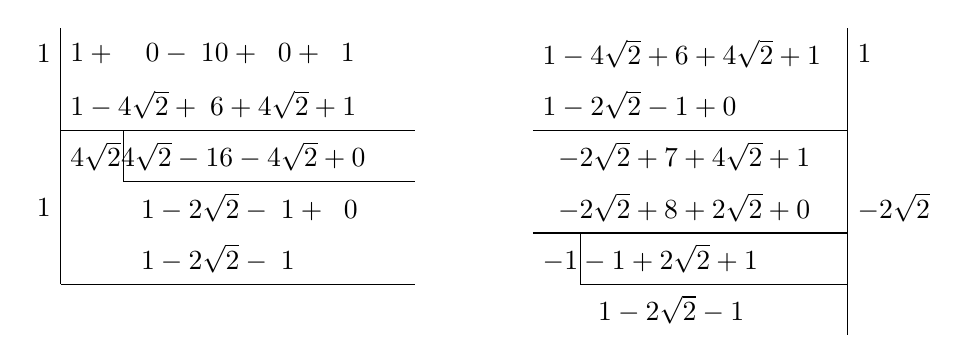
\begin{tikzpicture}[yscale=1.3]
\begin{scope}
\node at (0,0)[right]{$1+\quad 0-\; 10+\;\; 0+\;\; 1$};
\node at (0,-0.5)[right]{$1-4\sqrt{2}+\;6+4\sqrt{2}+1$};
\node at (0,-1)[right]{$4\sqrt{2} 4\sqrt{2}-16-4\sqrt{2}+0$};
\node at (0,-1.5)[right]{$\qquad\;\; 1-2\sqrt{2}-\;1+\;\;0$};
\node at (0,-2)[right]{$\qquad\;\; 1-2\sqrt{2}-\;1$};
\draw (0,.25)--(0,-2.25);
\draw (0,-.75)--(4.5,-.75);
\draw (.8,-.75)--(.8,-1.25)--(4.5,-1.25);
\draw (0,-2.25)--(4.5,-2.25);
\node at (0,0)[left]{1};
\node at (0,-1.5)[left]{1};
\end{scope}

\begin{scope}[xshift=6cm]
    \node at (0,0)[right]{$1-4\sqrt{2}+6+4\sqrt{2}+1$};
\node at (0,-0.5)[right]{$1-2\sqrt{2}-1+0$};
\node at (0,-1)[right]{$\;\;-2\sqrt{2}+7+4\sqrt{2}+1$};
\node at (0,-1.5)[right]{$\;\;-2\sqrt{2}+8+2\sqrt{2}+0$};
\node at (0,-2)[right]{$-1-1+2\sqrt{2}+1$};
    \node at (0,-2.5)[right]{$\qquad 1-2\sqrt{2}-1$};
\draw (4,.25)--(4,-2.75);
\draw(0,-.75)--(4,-.75);
\draw(0,-1.75)--(4,-1.75);
\draw(.6,-1.75)--(.6,-2.25)--(4,-2.25);
\node at (4,0)[right]{1};
\node at (4,-1.5)[right]{$-2\sqrt{2}$};
\end{scope}
\end{tikzpicture}
\end{center}
所以$\bigl(f(x),g(x)\bigr)=x^2-2\sqrt{2}x-1$。
\end{solution}


\begin{ex}
求$\bigl(f(x),g(x)\bigr)$:
\begin{enumerate}
    \item $f(x)=\poly{1,-7,13,3,-18}$
    
$g(x)=\poly{1,-5,2,20,-24}$
\item $f(x)=\poly{1,-7,-22,139,105}$
    
$g(x)=\poly{1,-8,-11,116,70}$
\item $f(x)=\poly{1,1,1,2},\quad g(x)=\poly{1,0,-1,-1}$
\end{enumerate}
\end{ex}

\section*{习题3.3}
\addcontentsline{toc}{subsection}{习题3.3}

\begin{enumerate}
    \item $f(x)=\poly{2,3,6,4,3},\quad g(x)=\poly{2,-5,-6,-12,-9}$

求:$\bigl(f(x),g(x)\bigr)$及$\bigl[f(x),g(x)\bigr]$。其中$\bigl[f(x),g(x)\bigr]$为$f(x)$与$g(x)$的最低公倍式。

\item $f(x)=\poly{2,3,-4,13,-6},\quad g(x)=\poly{2,-1,2,3,-2}$

$h(x)=\poly{1,3,1,5,6}$

求:$\bigl(f(x),g(x),h(x)\bigr)$

\item $f(x)=\poly{1,a,b,1},\qquad g(x)=\poly{1,b,a,1}$

求证:$(f,g)=1$,除非$a=b$或$a+b+2=0$。
\item $f(x)=\poly{2,-3,1},\qquad g(x)=\poly{3,-2,1}$

利用辗转相除法中关系式(3.15)的逆推,找出两个多项式$\mu(x)$, $\nu(x)$使下式成立:
\[\mu(x)\cdot f(x)+\nu(x)\cdot g(x)=(f,g)\]

\item $f(x)=\poly{2,-1,2},\qquad g(x)=\poly{1,1,1}$

试求两个多项式$\mu(x)$, $\nu(x)$使下式成立:
\[\mu(x)\cdot f(x)+\nu(x)\cdot g(x)=1\]

\item $m,n$是大于1的自然数,求$f(x)=x^m-1$及$g(x)=x^n-1$
的最高公因式。
\end{enumerate}


\section{插值公式}
如果$n$次多项式$f(x)$在取$n+1$个不同值时的函数值已给出,应用余式定理推论2就可以求出唯一的多项式函数$f(x)$. 在$f(x)$是一次多项式时,$y=ax+b$的图象是一条直线,推论2对于这个一次函数的论断的几何意义就是“两点确定一直线”。在一般情形下,一个$n$次多项式函数$y=f(x)$的曲线,由其所过的$n+1$个点所唯一确定,反之,仅给$n+1$个横坐标不同的点,总可以唯一确定一个次数不大于$n$的多项式函数$y=f(x)$的曲线。在数学中,这样的唯一性定理常常是计算问题解决问题的基本依据。这一节就讨论这样一些问题。

\subsection{余式定理推论的应用举例}
\begin{example}
    已知$f(2)=8$, $f(3)=f(4)=f(5)=0$, 求次数不大于3的多项式$f(x)$。
\end{example}

\begin{analyze}
如果设$f(x)=ax^3+bx^2+cx+d$, 用$x=2, 3,
4, 5$四个数相继代入,然后解四元一次方程组求出$a,b,c,d$. 虽然肯定可以求出来,但计算量太大。现已知中有有利条件:$f(3)=f(4)=f(5)=0$, 我们就可以应用因式定理把问题简化。
\end{analyze}

\begin{solution}
    由已知$f(3)=f(4)=f(5)=0$,因而可以
    设$f(x)=(x-3)(x-4)(x-5)q(x)$。
    
    由于$(x-3)(x-4)(x-5)$已是3次,而$f(x)$的次数
不大于3, 所以$q(x)$应为常数,即
\[f(x)=a_3(x-3)(x-4)(x-5)\]
再以$x=2$代入,得$3=-6a_3$,因此:$a_3=-\frac{1}{2}$

\[\therefore\quad f(x)=-\frac{1}{2}(x-3)(x-4)(x-5)\]
\end{solution}


\begin{example}
已知:$f_1(2)=3$, $f_1(3)=f_1(4)=f_1(5)=0$, $f_2(3)=6$, $f_2(2)=f_2(4)=f_2(5)=0$, $f_3(4)=-3$, $f_3(2)=f_3(3)=f_3(5)=0$, $f_4(5)=12$, $f_4(2)=f_4(3)=f_4(4)=0$

求四个次数不大于3的多项式$f_1(x)$, $f_2(x)$, $f_3(x)$, $f_4(x)$。
\end{example}

\begin{solution}
    解法同例3.21,可得
\[\begin{split}
    f_1(x)&=-\frac{1}{2}(x-3)(x-4)(x-5)\\
    f_2(x)&=3(x-2)(x-4)(x-5)\\
    f_3(x)&=\frac{3}{2}(x-2)(x-3)(x-5)\\
    f_4(x)&={2}(x-2)(x-3)(x-4)\\
\end{split}\]
\end{solution}

以上两例说明在已知函数值有若干个为零时,充分应用因式定理可以减少对待定系数的繁杂的计算量。(若一开始就令$f(x) =a_3a^3+a_2x^2+a_1x+a_0$, 就得解关于待定系数 $a_3,a_2,a_1,a_0$的四元一次方程组)。在已知函数值中没有零,或者很少为零的情况下,我们可以把所求的多项式$f(x)$分解为若干个多项式的和其中每一个多项式的函数值只有一个非零数。


\begin{example}
    已知$f(2)=3$, $f(3)=6$, $f(4)=-3$, $f(5)=12$, 求次数不大于3的多项式$f(x)$。
\end{example}

\begin{analyze}
    实际上$f(x)$正是例中四个多项式的和。
\end{analyze}

\begin{solution}
  令$f_1(x),f_2(x),f_3(x),f_4(x)$分别如例3.22中的已知条件所述,$F(x)=f_1(x)+f_2(x)+f_3(x)+f_4(x)$, 则
\[    F (2) =f_1 (2) +f_2 (2) +f_3 (2) +f_4 (2) =3+0+0+0=3\]

    同样可求得$F(3)=6$, $F(4)=-3$, $F(5)=12$, 可见:
\[\begin{split}
    f(x)=F(x)&=-\frac{1}{2} (x-3) (x-4)(x-5)+3 (x-2) (x-4)(x-5)\\
    &\qquad 
    +\frac{3}{2} (x-2) (x-3)(x-5)
   +2 (x-2) (x-3)(x-4)   
\end{split}\]    
\end{solution}



\begin{example}
    已知$\alpha_i\; (i=1, 2, 3, 4)$是四个两两不等的数。$c_i\; (i=1, 2, 3, 4)$是另外四个数。试求次数不大于3的多项式$f(x)$, 使得$f (\alpha_i) =c_i,\; (i=1, 2, 3, 4)$ 
\end{example}

\begin{solution}
    与例3.23的处理方法相类似,可假设四个多项式
$f_1(x),f_2(x),f_3(x),f_4(x)$,$f_i(\alpha_j)=\delta_{ij}c_i$    
    
    此处$$\delta_{ij}=\begin{cases}
        1,& i=j\\
        0,& i\ne j
    \end{cases}\quad  (i,j=1, 2, 3, 4)$$
则显然有$f(x)=f_1(x)+f_2(x)+f_3(x)+f_4(x)$.
还可以简记为$$f(x)=\sum^4_{i=1}f_i(x)$$
其中,$f_i(x)=k(x-\alpha_2)(x-\alpha_3)(x-\alpha_4)$

$\because\quad f_1(\alpha_1)=c_1$

$\therefore\quad k_1=\frac{c_1}{(\alpha_1-\alpha_2)(\alpha_1-\alpha_3)(\alpha_1-\alpha_4)}$

\[\therefore\quad f_1(x)=\frac{c_1(x-\alpha_2)(x-\alpha_3)(x-\alpha_4)}{(\alpha_1-\alpha_2)(\alpha_1-\alpha_3)(\alpha_1-\alpha_4)}\]
同理可求得:
\[\begin{split}
    f_2(x)&=\frac{c_2(x-\alpha_1)(x-\alpha_3)(x-\alpha_4)}{(\alpha_2-\alpha_1)(\alpha_2-\alpha_3)(\alpha_2-\alpha_4)}\\
    f_3(x)&=\frac{c_3(x-\alpha_1)(x-\alpha_2)(x-\alpha_4)}{(\alpha_3-\alpha_1)(\alpha_3-\alpha_2)(\alpha_3-\alpha_4)}\\
    f_4(x)&=\frac{c_4(x-\alpha_1)(x-\alpha_2)(x-\alpha_3)}{(\alpha_4-\alpha_1)(\alpha_4-\alpha_2)(\alpha_4-\alpha_3)}
\end{split}\]
因此:
\[\begin{split}
f(x)&=\frac{c_1(x-\alpha_2)(x-\alpha_3)(x-\alpha_4)}{(\alpha_1-\alpha_2)(\alpha_1-\alpha_3)(\alpha_1-\alpha_4)}+\frac{c_2(x-\alpha_1)(x-\alpha_3)(x-\alpha_4)}{(\alpha_2-\alpha_1)(\alpha_2-\alpha_3)(\alpha_2-\alpha_4)}\\
&\quad +\frac{c_3(x-\alpha_1)(x-\alpha_2)(x-\alpha_4)}{(\alpha_3-\alpha_1)(\alpha_3-\alpha_2)(\alpha_3-\alpha_4)}+\frac{c_4(x-\alpha_1)(x-\alpha_2)(x-\alpha_3)}{(\alpha_4-\alpha_1)(\alpha_4-\alpha_2)(\alpha_4-\alpha_3)}
\end{split}\]
还可以简单记为:
\[f(x)=\sum^4_{i=1} c_i\frac{(x-\alpha_1)(x-\alpha_2)\cdots (x-\alpha_{i-1})(x-\alpha_{i+1})\cdots (x-\alpha_4)}{(\alpha_i-\alpha_1)(\alpha_i-\alpha_2)\cdots (\alpha_i-\alpha_{i-1})(\alpha_i-\alpha_{i+1})\cdots (\alpha_i-\alpha_4)}\]
\end{solution}


\begin{example}
$\alpha_1,\alpha_2,\alpha_3$表三个两两不等的数,试用$f(\alpha_1)$, $f(\alpha_2)$, $f(\alpha_3)$来表示$(x-\alpha_1)(x-\alpha_2)(x-\alpha_3)$除多项式$f(x)$所得的余式。
\end{example}

\begin{solution}
\[f(x)=(x-\alpha_1)(x-\alpha_2)(x-\alpha_3)q(x)+r(x)\]
并且:${\rm deg}r(x)\le 2$或$r(x)=0$,则
\[r(\alpha_1)=f(\alpha_1),\qquad r(\alpha_2)=f(\alpha_2),\qquad r(\alpha_3)=f(\alpha_3)\]
 仿照上例可得:
 \[\begin{split}
     r(x)&=f(\alpha_1)\frac{(x-\alpha_2)(x-\alpha_3)}{(\alpha_1-\alpha_2)(\alpha_1-\alpha_3)} +f(\alpha_2)\frac{(x-\alpha_1)(x-\alpha_3)}{(\alpha_2-\alpha_1)(\alpha_2-\alpha_3)}
     \\
&\quad     +f(\alpha_3)\frac{(x-\alpha_1)(x-\alpha_2)}{(\alpha_3-\alpha_1)(\alpha_3-\alpha_2)}
 \end{split}\]
\end{solution}

\begin{ex}
\begin{enumerate}
    \item 已知$f(1)=f(2)=f(3)=2$, $f(0)=-16$。求三次多项式$f(x)$。
    \item 已知$f(-3)=42$, $f(-2)=6$, $f(-1)=0$, $f(0)=0$, $f(1)=6$。求四次多项式$f(x)$。
\end{enumerate} 
\end{ex}

\subsection{插值公式}

把上述例题所得的结果予以推广,应有
下列定理:

\begin{blk}{定理}
    设$f(x)$是一个次数不大于$n$的多项式,$\alpha_i\; (i=1, 2,\ldots,n,n+1)$表示$n+1$个两两不等的数,$b_i\; (i=1, 2,\ldots,n,n+1)$是任意$n+1$个数,而且
$f (\alpha_i) =b_i,\; (i=1, 2,\ldots,n,n+1)$,则:
\[\begin{cases}
   f(x)=\sum^{n+1}_{i=1} f_i(x)\\
   f_i(x)=b_i\frac{(x-\alpha_1)\cdots(x-\alpha_{i-1})(x-\alpha_{i+1})\cdots (x-\alpha_{n+1})}{(\alpha_i-\alpha_1)\cdots(\alpha_i-\alpha_{i-1})(\alpha_i-\alpha_{i+1})\cdots (\alpha_i-\alpha_{n+1})}
\end{cases}\]
\end{blk}

\begin{proof}
令$f_i(x)$是由下列条件所唯一确定的次数不大于$n$的多项式:
\[f_i(\alpha_j)=\delta_{ij}b_i,\qquad \delta_{ij}=\begin{cases}
    1&i=j\\
    0&i\ne j
\end{cases}\quad (i,j=1,2,\ldots,n+1)\]
则由因式定理可知
\[f_i(x)=c_i(x-\alpha_1)\cdots(x-\alpha_{i-1})(x-\alpha_{i+1})\cdots (x-\alpha_{n+1})\]
由$f_i(\alpha_i)=b_i$定出$c_i$的值,可得
\[c_i=\frac{b_1}{(\alpha_i-\alpha_1)\cdots(\alpha_i-\alpha_{i-1})(\alpha_i-\alpha_{i+1})\cdots (\alpha_i-\alpha_{n+1})}\]
$\therefore\quad f_i(x)=b_i\frac{(x-\alpha_1)\cdots(x-\alpha_{i-1})(x-\alpha_{i+1})\cdots (x-\alpha_{n+1})}{(\alpha_i-\alpha_1)\cdots(\alpha_i-\alpha_{i-1})(\alpha_i-\alpha_{i+1})\cdots (\alpha_i-\alpha_{n+1})}$

显然有 $f(x)=\displaystyle\sum^{n+1}_{i=1} f_i(x)$.
\end{proof}

上述公式叫做拉格朗日的插值公式。

\begin{example}
   令$g_n(x)$为一个$n$次多项式,它在$0, 1,\ldots,n-1,n $时的值分别为$0, 0,\ldots,0, 1$, 求$g_n(x)$. 
\end{example}

\begin{solution}
    由插值公式直接得出
    \[\begin{split}
        g_n(x)&=\frac{x(x-1)(x-2)\cdots(x-n+1)}{1\cdot 2\cdots n}\\
        &=\frac{x(x-1)\cdots(x-n+1)}{n!}      
    \end{split}\]

$n!$对非负整数$n$都有定义,读作“$n$阶乘”,当$n>0$时,
$n!=1\x2\x\cdots \x n$, 并规定$0!=1$.

注意$g_n(x)$是应用插值公式最容易求出的多项式,我们以后将会有意识地引进这样的多项式。
\end{solution}

\begin{example}
    已知$f(x)$是一个次数不大于3的多项式,$f(0)=1$, $f(1)=4$, $f(2)=15$, $f(3)=40$, 不求出$f(x)$, 直接计算$f(1.5)$.
\end{example}

\begin{solution}
    由插值公式可知
    \[\begin{split}
         f (1. 5) &=1\cdot \frac{(1. 5-1) (1.5-2)(1.5-3)}{(0-1) (0-2)(0-3)}+4\cdot \frac{(1.5-0)(1.5-2)(1.5-3)}{(1-0) (1-2)(1-3)}\\
         &\quad +15\cdot \frac{(1. 5-0) (1.5-1)(1.5-3)}{(2-0) (2-1)(2-3)} +40\cdot \frac{(1. 5-0) (1.5-1)(1.5-2)}{(3-0) (3-1)(3-2)}\\
         &=8.125
    \end{split}\]
\end{solution}
 

\begin{example}
某人身旁没有三角函数表(或带有三角函数的计算器),却需要计算$\sin23^{\circ}$, 他记得一些特殊角的三角函数:
\[\sin0^{\circ}=0,\qquad \sin15^{\circ}=\frac{1}{4} (\sqrt{6}-\sqrt{2}) =0. 259,\qquad \sin30^{\circ}=0.5\]
\[\sin45^{\circ}=\frac{\sqrt{2}}{2}=0. 707,\qquad \sin60^{\circ}=\frac{\sqrt{3}}{2}=0.866\]
他根据这些数据把函数$y=f(x)=\sin x$近似地看成一个次数不大于4的多项式,问如此计算出来的$\sin23^{\circ}$是多少?
\end{example}

\begin{solution}
    由已知$f(0)=0$, $f(15)=0. 259$, $f(30)=0. 5$, $f(45)=0. 707$, $f(60)=0. 866$, 求$f(23)$。

方法同例3.26
\[\begin{split}
    f(23)&=0. 259\x \frac{23 (23-30) (23-45)(23-60)}{15 (15-30) (15-45)(15-60)}\\
    &\quad +0. 5\x \frac{23 (23-15) (23-45)(23-60)}{30 (30-15) (30-45)(30-60)}\\
&\quad +0. 707\x \frac{23 (23-15) (23-30)(23-60)}{45 (45-15) (45-30)(45-60)}\\
&\quad +0.866\x \frac{23 (23-15) (23-30)(23-45)}{60 (60-15) (60-30)(60-45)}\\
&\approx \frac{23}{15^4}\x (246+814-244+44) \approx 0. 391
\end{split}\]

实际上从三角函数表上査出的 $\sin23^{\circ}$如果要求精确到0.001也是0.391.
\end{solution}

关于一个函数为什么可以近似地用多项式来代替,在什么条件下才可以近似地用多项式来代替,我们到学习微积分时再加以研究。这里只说明插值公式有这样一个“插值”的应用。

\begin{ex}
    \begin{enumerate}
    \item 已知$f(0)=0$, $f(1)=1$, $f(2)=2$, $f(3)=3$,
    $f(4)=4$, 试求一个次数不大于4的多项式$f(x)$。
    \item 已知$f(0)=0$, $f(1)=1$, $f(2)=2$, $f(3)=3$,
    $f(4)=4$, 若求一个多项式$f(x)$, 没有说明其次数不大于4, 能否得出$f(x)=x$的结论?为什么?举一个反例。
    \item 已知$f(x)$是一个二次多项式,$f(1)=3$, $f(2)=6$, $f(8)=13$, 计算$f(1. 5)$。
    \item 为了计算$\sqrt{26}$, 只记得$\sqrt{2}=1. 414$, $\sqrt{3}=1. 732$, 因而算得$\sqrt{24}=4.898$, $\sqrt{25}=5$, $\sqrt{27}=5. 196$, 试由这三个数据近似地计算出$\sqrt{26}$(精确到0.001)。
    \end{enumerate} 
    \end{ex}
    
    \section*{习题3.4}
    \addcontentsline{toc}{subsection}{习题3.4}
    \begin{enumerate}
        \item 已知$f(4)=0$, $f(6)=-12$, $f(7)=-20$,
        $f(8)=-18$, 求次数尽可能小的多项式$f(x)$, 然后计算$f(12)$。
        \item 当$x=2, 3, 4, 5$时,$f(x)$的值分别为$5, 4,-7,-34$, 求三次多项式$f(x)$。
        \item 已知$5x^2+19x+18=\frac{a}{2}(x-2)(x-3)-b(x-3)(x-1)+\frac{c}{2}(x-1)(x-2)$, 计算$a,b,c$这三个数
        对多项式$5x^2+19x+18$ 来说有些什么意义?
        \item $a,b,c$是两两不等的三个数,已知$f(a)=bc$, $f(b)=
        ca$, $f(c)=ab$, 求次数不超过2的多项式$f(x)$。
        \item $a,b,c$是两两不等的三个数,已知$f(a)=b+c$, $f(b)=
        c+a$, $f(c)=a+b$, 求次数不超过2的多项式$f(x)$。
    \end{enumerate}
    
    \section{多项式的导数与换元展开式}
    在本节里,我们将引进多项式的导数概念及其简单性质。并学习多项式的换元展开式,进一步把余式定理推广,为今后研究多项式函数在某定点邻近的区域内的局部性质打下一定基础。
    
    \subsection{多项式的导数}
    导数概念是微积分学中的重要概
    念,这里仅就多项式来讨论,我们规定:
    
\begin{blk}{定义1}
对任意的非负整数$n$, 单项式$ax^n$
的导数就是单项式$nax^{n-1}$.
\end{blk}    

     
\begin{blk}{定义2}
对任意的非零多项式
$f (x) =a_nx^n+a_{n-1}x^{n-1}+\cdots+a_1x+a_0$
的导数就是各项导数的代数和,记作
\[f' (x) =na_nx^{n-1}+(n-1)a_{n-1}x^{n-2}+\cdots +a_1\]

同样,$f'(x)$的导数,记作
\[f'' (x) =n (n-1) a_nx^{n-2} + (n-1) (n-2)a_{n-1}x^{n-3}+\cdots+a_2\]
叫做多项式$f(x)$的二阶导数;
$f''(x)$的导数,记作$f'''(x)$,叫做$f(x)$的三阶导数,也是$f'(x)$的二阶导数;一般地,$f'(x)$的$k-1$阶导数,就是
$f(x)$的$k$阶导数,记作$f^{(k)}(x)$,即:
\[\left[f^{(k-1)} (x)\right]'=f^{(k)}(x)\]
\end{blk}    

   \begin{example}
    求 $f(x)=2x^3-8x^2+5x-4$的各阶导数.
    \end{example}

    \begin{solution}
\[\begin{split}
    f' (x) &=6x^2-16x+5\\
        f'' (x) &=12x-16\\
        f''' (x) &=12\\
        f'''' (x) &=f^{(5)}(x)=\cdots =f^{(n)}(x)=0,\qquad (n\ge 4)
\end{split}\]
    \end{solution}    

    显然,一元$n$次多项式的$n$阶导数是一个非零常数(零次多项式),从$n+1$阶系数开始,以后各高阶导数都是零;
    特别地,零次多项式的导数等于零;而零多项式的各阶导数仍是零。

    总之,多项式的导数仍然是多项式。而且对于系数在整数,有理数,实数范围内的各多项式集合,求导数这种运算也是封闭的。

 
    \begin{example}
求多项式$f (x) =a_3x^3+a_2x^2+a_1x+a_0\quad  (a_3\ne 0)$ 的各阶导数,并求出各阶导数在$x=x_0$时的值。          
    \end{example}           
         
    \begin{solution}
\[\begin{split}
 f'(x)&=3a_3x^2+2a_2x+a_1\qquad 
    f' (x_0) =3a_3 x^2_0 +2a_2x_0+a_1\\
    f'' (x) &=6a_3x+2a_2\qquad \qquad \quad 
    f'' (x_0) =6a_3x_0+2a_2\\
    f''' (x) &=6a_3\qquad \qquad \qquad \qquad 
     f''' (x_0 ) =6a_3\\
     f^{(4)} (x)&=f^{(5)}(x)=\cdots =f^{(n)}(x)=0\\
     f^{(4)}  (x_0)&=f^{(5)}(x_0)=\cdots =f^{(n)}(x_0)=0 
\end{split}\] 
    \end{solution} 

容易证明,多项式的导数有以下性质:

\begin{blk}{性质1}
    多项式$f(x)$与常数$k$乘积的导数等于$f(x)$的导数与$k$的乘积,即
\[[kf (x) ]'=k\cdot f' (x) \]
\end{blk}   

\begin{proof}
设$f(x)=a_nx^n+a_{n-1}x^{n-1}+\cdots+a_1x+a_0$,
则
\[kf(x)=ka_nx^n+ka_{n-1}x^{n-1}+\cdots+ka_1x+ka_0\]
因此:
\[\begin{split}
    [kf(x)]'&=kna_nx^{n-1}+k(n - 1)a_{n-1}x^{n-2}+\cdots+ka_1\\
&=k \left[na_nx^{n-1}+(n - 1)a_{n-1}x^{n-2}+\cdots+a_1\right]\\
&=kf' (x) 
\end{split}\]
\end{proof}

\begin{blk}{性质2}
    两多项式$f(x),g(x)$和的导数等于这两个多项式的导数和,即
\[[f (x) +g (x) ]'=f' (x) +g' (x) \]  
\end{blk}  
 
\begin{proof}
设$f(x)=a_nx^n+a_{n-1}x^{n-1}+\cdots+a_1x+a_0$,$g(x)=b_mx^m+b_{m-1}x^{m-1}+\cdots+b_1x+b_0$,不失一般性,不妨设$n>m$,则有
\[f(x)+g(x)=a_nx^n+\cdots + (a_{m}+b_m)x^{m}+\cdots+(a_1+b_1)x+a_0+b_0\]
因此:
\[\begin{split}
    [f(x)+g(x)]'&=na_nx^{n-1}+\cdots + m(a_{m}+b_m)x^{m-1}+\cdots+a_1+b_1\\
    &=(na_nx^{n-1}+\cdots+ma_mx^{m-1}+\cdots +a_1)+(mb_mx^{m-1}+\cdots +b_1)\\
    &=f'(x)+g'(x)
\end{split}\]
\end{proof}  

综合性质1, 2, 就可以得出:对任意的两个常数$\mu$, $\lambda$和多项式$f(x),g(x)$, 下述等式是成立的,即
\[[\mu\cdot f (x) +\lambda\cdot g (x) ]'=\mu f' (x) +\lambda g' (x) \]

\begin{blk}{性质3}
两个多项式$f(x),g(x)$的乘积的导数等于$f(x)$的导数乘以$g(x)$与$g(x)$的导数乘以$f(x)$的和,即
\[[f (x) g (x) ]'=f' (x) g (x) +g' (x) f (x) \]
\end{blk}

\begin{blk}{性质4}
    一个多项式$f(x)$的$m$次方的导数为
\[[f^m (x) ] '= mf^{m-1} (x) f' (x) \]
\end{blk}

性质3, 4的证明亦可以像前两个性质一样通过实际计算进行,但较繁,这里略去不证,同学们可通过练习验证。

\begin{example}
求下列多项式的导数:
\begin{enumerate}
    \item $f(x)=g(x)h(x)$
    \item $f (x) =g^2 (x) +2g (x) h (x) +h^2 (x) $
\end{enumerate} 
这里$g(x)=3x^2-1$, $h (x) =8x^3+2x-1$
    \end{example}

    \begin{solution}
\begin{enumerate}
    \item $f(x)=(3x^2-1)(8x^3+2x-1)$
\[\begin{split}
    f' (x) &= (3x^2-1)' (8x^3+2x-1)+(8x^3+2x-1)' (3x^2-1) \\
    &=6x (8x^3+2x-1) + (24x^2+2) (3x^2-1)\\
    &=48x^4+12x^2-6x+72x^4-18x^2-2\\
    &=120x^4-6x^2-6x-2
\end{split}\]
    \item $f(x)=g^2 (x) +2g (x) h (x) +h^2 (x) =[g(x)+h(x)]^2=(8x^3+3x^2+2x-2)^2$
\[\begin{split}
    f'(x)&=2(8x^3+3x^2+2x-2)(8x^3+3x^2+2x-2)'\\
    &=2(8x^3+3x^2+2x-2)(24x^2+6x+2)\\
    &=\poly{384,240,164,-60,-16,-8}
\end{split}\]
\end{enumerate}
 \end{solution}
           
\begin{ex}
\begin{enumerate}
    \item 求下列各多项式的各阶导数
\begin{multicols}{2}
\begin{enumerate}
    \item $f (x) =3x^2+x-2$
    \item $f(x) =ax^2+bx+c$
    \item $f(x)=\frac{4\cdot 3}{2!}a^2x^2$
\end{enumerate}
\end{multicols}

    \item 对于$f(x)=a_3x^3+a_2x^2+ax+a_0,\quad g(x)=b_2x^2+b_1x+b_0$
    
    验证导数的性质3是成立的。

    \item 求下列各多项式的导数:
\begin{multicols}{2}
\begin{enumerate}
    \item $f (x) =\varphi^2 (x) +1$
    \item $f(x)=\varphi(x)g(x)$
    \item $f (x) =\varphi^3 (x) g (x)$
    \item $f(x)=\varphi^2(x)-g^2(x)$
\end{enumerate}
\end{multicols}
这里$\varphi(x)=x-2,\quad g(x)=3x^3+5x-1$.
    \item 试试看:你能证明“如果$(x-a)^k$能够整除$f(x)$, 那么$(x-a)^{k-1}$一定能够整除$f'(x)$吗”?
\end{enumerate}
\end{ex}
 
\subsection{多项式的换元展开式——泰勒公式}

 在初中代数
中,我们曾经学习过用综合除法的方法,将任一个非零次多项式$f(x)$展开成$(x-a)$的幂的形式。如果令$x-a=t$则$x=a+t$将它代入$f(x)$后,即可将$f(x)$展开成元$t=(x-a)$的幂的形式,按升幂排列成:
\[f (x) =f (a+t) =c_0+c_1t+c_2t^2+\cdots+c_nt^n\]
就叫做多项式$f(x)$在$x=a$点的换元展开式。

这里的待定系数$c_i,\; (i=0, 1, 2,\ldots,n)$ 显然只与$f(x)$
和所选定的点$a$有关。以下我们就复习用综合除法确定这些系数的方法,并进一步研究这些系数的一般规律,得出一般公式。

    \begin{example}
        用综合除法,将$f (x) =2x^2-x-2$展开成$x-1$的幂的形式。
    \end{example}    
    
    \begin{solution}
  用$x-1$去连续除$f(x)$, 由综合除法得
\begin{center}
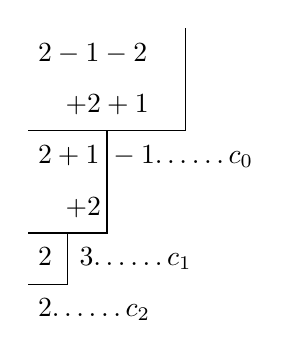
\begin{tikzpicture}[yscale=1.3]
    \node at (0,0)[right]{$2-1-2$};
    \node at (0,-0.5)[right]{$\quad +2+1$};
    \node at (0,-1)[right]{$2+1\; -1 $……$c_0$};
    \node at (0,-1.5)[right]{$\quad +2$};
    \node at (0,-2)[right]{$2\quad 3$……$c_1$};
    \node at (0,-2.5)[right]{$2$……$c_2$};
\draw (0,-.75)--(2,-.75)--(2,.25);
\draw (0,-1.75)--(1,-1.75)--(1,-.75);
\draw (0,-2.25)--(.5,-2.25)--(.5,-1.75);
\end{tikzpicture}
\end{center}

\[\therefore\quad f (x) =-1+3 (x-1) +2 (x-1)^2\]
或
\[f (1+t) =-1+3t+2t^2,\qquad (x-1=t)\]
\end{solution}
   
\begin{example}
已知$f(x)=a_3x^3+a_2x^2+a_1x+a_0$, 试求:
\begin{multicols}{2}
\begin{enumerate}
    \item $f (1+t)$
    \item $f(x_0+t)$
\end{enumerate}
\end{multicols}
\end{example}

\begin{solution}
\begin{enumerate}
    \item 
这就是要求当$x=1+t$, 即$t=x-1$时$f(x)$的换元展开,可以用综合除法
\begin{center}
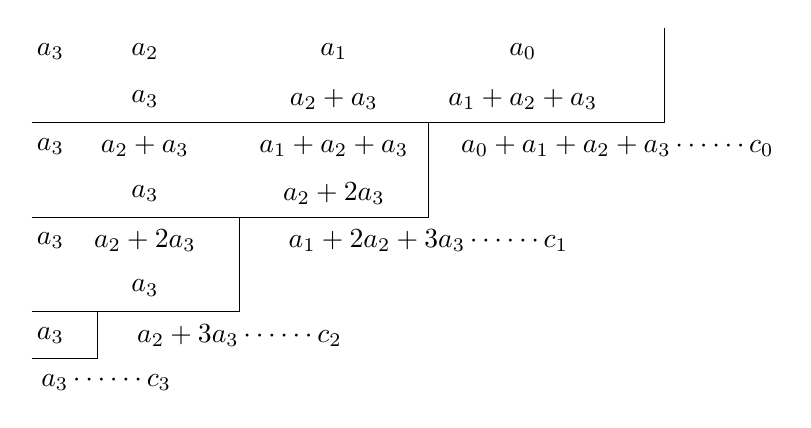
\begin{tikzpicture}[scale=1.2]
\foreach \x/\xtext in {0/a_3,1/a_2,3/a_1,5/a_0}
{
    \node at (\x,0){$\xtext$};
}
\foreach \x/\xtext in {0/{},1/a_3,3/a_2+a_3,5/a_1+a_2+a_3}
{
    \node at (\x,-0.5){$\xtext$};
}
\foreach \x/\xtext in {0/a_3,1/a_2+a_3,3/a_1+a_2+a_3,6/a_0+a_1+a_2+a_3\cdots\cdots c_0}
{
    \node at (\x,-1){$\xtext$};
}
\draw(-.2,-.75)--(6.5,-.75)--(6.5,.25);
\foreach \x/\xtext in {1/a_3,3/a_2+2a_3}
{
    \node at (\x,-1.5){$\xtext$};
}
\draw(-.2,-1.75)--(4,-1.75)--(4,-.75);
\foreach \x/\xtext in {0/a_3,1/a_2+2a_3,4/a_1+2a_2+3a_3\cdots\cdots c_1}
{
    \node at (\x,-2){$\xtext$};
}
\node at (1,-2.5){$a_3$};
\draw(-.2,-2.75)--(2,-2.75)--(2,-1.75);
\foreach \x/\xtext in {0/a_3,2/a_2+3a_3\cdots\cdots c_2}
{
    \node at (\x,-3){$\xtext$};
}
\node at (-.2,-3.5)[right]{$a_3\cdots\cdots c_3$};
\draw(-.2,-3.25)--(.5,-3.25)--(.5,-2.75);

\end{tikzpicture}
\end{center}
因此:
\[\begin{split}
    f (x) &= (a_0+a_1 +a_2 +a_3) + (a_1 +2a_2+3a_3 ) (x-1)\\
    &\qquad +(a_2 +3a_3) (x-1)^2+a_3(x-1)^3\\
f(1+t)&=(a_0+a_1 +a_2 +a_3) +(a_1 +2a_2+3a_3)t \\
&\qquad + (a_2+3a_3) t^2+a_3t^3
\end{split}\]

\item 直接换元,令$x=x_0+t$代入$f(x)$, 并展开整理成$t$
的升幂排列形式
\[\begin{split}
    f (x_0+t) &=a_3(x_0+t) +a_2(x_0+t)^2+a_1(x_0+t)+a_0\\
&=(a_0 +a_1x_0 +a_2x_0^2+a_3x_0^3) + (a_1+2a_2x_0+3a_3 x^2_0)t\\
&\qquad + (a_2+3a_3x_0) t^2+a_3t^3
\end{split} \]
\end{enumerate}
\end{solution}

为了找出换元展开式中待定系数$c_i\; (i=0, 1,\ldots,n)$的一般规律,我们对例3.33(2)分析并验证如下:

换元展开式中的常数项$a_0+a_1x_0+a_2x_0^2+a_3x_0^3$正好是$x=x_0$时,多项式$f(x)$的值$f(x_0)$. 例3.32及例3.33(1)也是 如此;$c_0=f (x_0)$。

换元展开式中的一次项系数 $a_1+2a_2x_0+3a_3x_0^2$正好是$x=x_0$时多项式$f(x)$的导数$f'(x)=3a_3x^2+2a_2x+a_1$的值$f'(x_0)=a_1+2a_2x_0+3a_3x_0^2$。例3.32及例3.33(1)也是如此;
$c_1 =f' (x_0)$。

换元展开式中的二次项系数 $a_2+3a_3x_0$正是$x=x_0$时,
$f(x)$的二阶导数$f'(x)=6a_3x+2a_2$的值的一半:$\frac{1}{2}f''(x_0)=a_2+3a_3x_0$。例3.32及例3.33(1)也是如此;$c_2=\frac{1}{2}f''(x_0)$。

换元展开式中的三次项系数$c_3$, 也容易分析出它正是当$x=x_0$时,$f(x)$的三阶导数$f'''(x)=6a_1$的值的六分之一,$\frac{1}{6}f'''(x_0)=a_3$, 可验证例3.33(1)也是如此;
$c_3=\frac{1}{6}f''' (x_0)$。

这样一来,利用导数概念,换元展开式就可以写成:
\[f(x_0+t)=f(x_0)+f'(x_0)t+\frac{1}{2}f''(x_0)t^2+\frac{1}{6}f'''(x_0)t^3\]    
进而可写成更有规律、便于记忆的形式
\[f(x_0+t)=f(x_0)+\frac{f'(x_0)}{1!}t+\frac{f''(x_0)}{2!}t^2+\frac{f'''(x_0)}{3!}t^3\]    
同样,例3.33(1)的换元展开写成
\[f (1+t) =f (1) +\frac{f'(1)}{1!}t+\frac{f''(1)}{2!}t^2+\frac{f'''(1)}{3!}t^3\]
例3.32 也可以写成
\[f (1+t) =f (1) +\frac{f'(1)}{1!}t+\frac{f''(1)}{2!}t^2=-1+3t-2t^2\]

实际上,这正是多项式换元展开式的一般规律,推广到$n$次多项式就得到重要的泰勒定理。
    
\begin{blk}{定理(泰勒定理)}
 一元$n$次多项式$f(x)$在点$x_0$
的换元展开式为
\begin{equation}
    f(x_0+t)=f(x_0)+\frac{f'(x_0)}{1!}t+\frac{f''(x_0)}{2!}t^2+\cdots+\frac{f'''(x_0)}{n!}t^n
\end{equation}   
\end{blk}

定理的一般证明这里略去,但容易验证,这个定理的内容对于零多项式、零次多项式都是适合的;对二、三次多项式我们从例3.32和例3.33也已验证过是适合的,对于其它高次多项式以后再给出确切证明,现在可以应用。

    \begin{example}
已知$f(x)=\poly{1,0,-2,3,5}$,试求$f(x)$在$x=1$点的展开式。    
    \end{example}    
    
    \begin{solution}
\begin{center}
\begin{tabular}{lll}
$f(x)=\poly{1,0,-2,3,5}$  &  $f(1)=7$  \\
$f'(x)=\poly{4,0,4,3}$  &  $f'(1)=3$  \\
$f''(x)=\poly{12,0,-4}$  &  $f''(1)=8$& $\frac{8}{2}=4$  \\
$f'''(x)=24x$  &  $f'''(1)=24$ & $\frac{24}{3!}=4$\\
$f''''(x)=24$  &  $f''''(1)=24$ & $\frac{24}{4!}=1$\\
\end{tabular}    
\end{center}

$\therefore\quad f(1+t)=7+3t+4t^2+4t^3+t^4$。又由于$x=a+(x-a)$,因此:
\begin{equation}
    \begin{split}
    f(x)&=f[a+(x-a)]\\
    &=f(a)+\frac{f'(a)}{1!}(x-a)+\frac{f''(a)}{2!}(x-a)^2+\cdots+\frac{f^{(n)}(a)}{n!}(x-a)^n
\end{split}
\end{equation}
(3.17)式叫做多项式$f(x)$在点$x=a$的换元展开式。
    \end{solution}

(3.16)与(3.17)本质上是相同的,都叫做泰勒公式,只是(3.16)式中的$t$相当于(3.17)式中的$x-a$罢了,不过在今后应用更多的是(3.17)式。

 \begin{example}
    已知$f(x)=x^5+2x^4-2x^3+7x-5$, 试将$f(x)$展开成$x+1$的升幂多项式。
    \end{example}

    \begin{solution}    
\begin{center}
\begin{tabular}{lll}
$f(x)=\poly{1,2,-1,0,7,-5}$  &  $f(-1)=-10$  \\
$f'(x)=\poly{5,8,-3,0,7}$  &  $f'(-1)=1$  \\
$f''(x)=\poly{20,24,-6,0}$  &  $f''(-1)=10$& $\frac{10}{2!}=5$  \\
$f'''(x)=\poly{60,48,-6}$  &  $f'''(-1)=6$ & $\frac{6}{3!}=1$\\
$f^{(4)}(x)=120x+48$  &  $f^{(4)}(-1)=-72$ & $\frac{-72}{4!}=-3$\\
$f^{(5)}(x)=120$  &  $f^{(5)}(-1)=120$ & $\frac{120}{5!}=1$\\
\end{tabular}    
\end{center}
          
$\therefore\quad f(x)=-10+(x-1)+5(x-1)^2+(x-1)^3-3(x-1)^4+(x-1)^5$
    \end{solution}

    还可以用连续作综合除法的方法,得出同样的结果。同学们可以验证一下。

\begin{ex}
\begin{enumerate}
    \item 试用秦勒公式将下列多项式在给定点展开成升幂形式:
\begin{enumerate}
    \item $g(x)=\poly{7,-3,4,-1}$,在$x=2$点;
    \item $f (x) =9x^5-188$,在$x=-2$点;
    \item $h(x)=x^4-x^2-1$,在$x=-1$点。
\end{enumerate}

    \item 试用泰勒公式将下列多项式展开成指定一次式的升幂形式:
\begin{enumerate}
    \item $f(x)=2x-2x^2+x^3$, 展成$x-1$的幂;
    \item $g(x)=2x^3+24x^2+34x+30$, 展成$x+2$的幂;
    \item $h(x)=28x-27+x^3-9x^2$展成$x-3$的幂。
\end{enumerate} 
\end{enumerate}
\end{ex}
    
\subsection{余式定理的推广}

泰勒公式,实际上就是通过多
项式的恒等变形,把一个以$x$为元的多项式变换为一个以
$x-a$为元的升幂多项式。

有了泰勒公式,我们可以更深刻,更一般地去理解余式定理。

由泰勒公式
\[f(x)=f(a)+\frac{f'(a)}{1!}(x-a)+\frac{f''(a)}{2!}(x-a)^2+\cdots+\frac{f^{(n)}(a)}{n!}(x-a)^n\]
可以直观看出:
\begin{enumerate}
    \item 若用$x-a$去除$f(x)$, 所得余式为$r_1(x)=f(a)$, 这正是我们在第二节所学的余式定理的内容;
    \item 若用$(x-a)^2$去除$f(x)$, 所得的余式为
    \[ r_2(x) =f (a) +\frac{f'(a)}{1!}  (x-a)\]
    这就要比余式定理的内容进一步了;
    \item 一般地,若用$(x-a)^k\; (k\le n)$除$f(x)$, 所得的余式为
    \[r_k(x)=f(a)+\frac{f'(a)}{1!}(x-a)+\cdots+\frac{f^{(k-1)}(a)}{(k-1)!}(x-a)^{k-1}\]
    这就是余式定理推广的结论。
\end{enumerate}

    \begin{example}
试求$f(x)=\poly{1,0,-2,8,5}$除以$g(x)=(x-1)^3$所得的余式$r(x)$。
    \end{example}    
    
    \begin{solution}
\begin{center}
\begin{tabular}{lll}
$f(x)=\poly{1,0,-2,8,5}$  &  $f(1)=12$  \\
$f'(x)=\poly{4,0,-4,8}$  &  $f'(1)=8$  \\
$f''(x)=\poly{12,0,-4}$  &  $f''(1)=8$& $\frac{8}{2!}=4$  \\
\end{tabular}    
\end{center}
          
$\therefore\quad f(x)$除以$g(x)$所得的余式为
\[\begin{split}
    r(x)&=f(1)+\frac{f'(1)}{1!}(x-1)+\frac{f''(1)}{2!}(x-1)^2\\
    &=12+8(x-1)+4(x-1)^2\\
    &=12-8+8x+4x^2-8x+4\\
    &=4x^2+8
\end{split}\]
    \end{solution}

    \begin{example}
已知一个首项系数是2的三次多项式 $g(x)$除以$(x-2)^3$所得的余式为$2x^2+x-1$, 试求这个多项式$g(x)$。
    \end{example}    
    
    \begin{solution}
设$g(x)=f(2)+\frac{f'(2)}{1!}(x-2)+\frac{f''(2)}{2!}(x-2)^2+\frac{f'''(2)}{3!}(x-2)^3$

由已知,$g(x)$的首项(最高次项)系数为2, 可得
\[\frac{f'''(2)}{3!}=2\quad \Rightarrow\quad f'''(2)=12\]

又由$g(x)$除以$(x-2)^3$所得余式为$2x^2+x-1$, 可以
得       
\[f(2)+\frac{f'(2)}{1!}(x-2)+\frac{f''(2)}{2!}(x-2)^2=2x^2+x-1\]
即:
\[\frac{1}{2}f''(2)x^2+[f'(2)-2f''(2)]x+[f(2)-2f'(2)+2f''(2)]=2x^2+x-1\]
 
根据多项式恒等的定义,可得:
\[\begin{cases}
    \frac{1}{2}f''(2)=2\\
    f'(2)-2f''(2)=1\\
    f(2)-2f'(2)+2f''(2)=-1
\end{cases}\]
解出方程组,得:
\[f''(2)=4,\qquad f'(2)=9,\qquad f(2)=9\]

因此:
\[\begin{split}
    g(x)&=9+9(x-2)+\frac{4}{2!}(x-2)^2+\frac{12}{3!}(x-2)^3\\
    &=9+9(x-2)+2(x-2)^2+2(x-2)^3\\
    &=2x^3-10x^2+25x-17
\end{split}\]
   \end{solution}


\begin{ex}
\begin{enumerate}
    \item 试求$f(x)=x^4+x^3+x+1$除以下列各式所得的余式分别是什么?
\[x-1;\quad  (x-1)^2;\quad (x-1)^3;\quad (x-1)^4\]
\item 已知$f(x)$的首项系数为3, ${\rm deg}f(x)=4$, 而且$f(x)$
分别除以$(x+2)$, $(x+2)^2$, $(x+2)^3$, $(x+2)^4$所得余式的常数项各是$-5,-13,-25,-41$, 试求$f(x)$。
\item 多项式 $x^4+ax^3-3x^2+bx+3$ 除以$(x-1)^2$所得的
余式为$x+1$, 试求$a,b$的值。
\end{enumerate}
\end{ex}


\section*{习题3.5}
\addcontentsline{toc}{subsection}{习题3.5}
\begin{enumerate}
    \item 求下列多项式的一、二、三阶导数:
\begin{enumerate}
    \item $f(x)=\poly{7,0,5,0,3,1}$
    \item $g(x)=x^n+x^{n-1}+x^{n-2}+x^{n-3}-4,\quad (n\ge 3)$
    \item $h(x)=4!x^4-3!x^3-2!x^2-1!x-0!$
\end{enumerate}
\item 已知$f(2)=(x-2)^2+1$, $g(x)=(x^2+\sqrt{2})^3$.
试求下列各多项式的导数:
\begin{multicols}{2}
\begin{enumerate}
    \item $f(x)+g(x)$
    \item $g (x) -f (x)$
    \item $f (x) g (x)$
    \item $g^n(x)$
\end{enumerate}
\end{multicols}

\item 已知$f(x)=(x+1)^3(2x-1)$, 试求:
\begin{multicols}{2}
    \begin{enumerate}
        \item $f'(x)$
        \item $\big(f(x),f'(x)\big)$
    \end{enumerate}
    \end{multicols}
\item 已知$f(x)=a_nx^n+a_{n-1}x^{n-1}+\cdots+a_x+a_0$, 
$g(x)=bx^m,\quad (a,b\ne 0)$。

求证:$[f(x)g(x)]'=f'(x)g(x)+g'(x)f(x)$

\item 试求$f(x)=(x-a)(x-b)(x-c)$的一阶导数。
\item 将下列多项式展开成指定的一次式的幂的形式:
\begin{enumerate}
\item $f(x)=10x^4-12x^3-9x^2-2x-1$, 展成$x-1$
的幂;
\item $y(x)=7x^5+1$, 展成$x+2$的幂。
\end{enumerate}

\item 如果$f(x)$分别除以$x-3$, $(x-3)^2$, $(x-3)^3$所得的
余式各为$2$, $2x-4$, $x^2-4x+5$, 且$f(x)$的首项系数为$\frac{1}{2}$, 试求f(x)。
\item 求f(x):
\begin{enumerate}
\item 已知$f'(x)=10x^4-12x^3-9x^2-2x-1$, 
且$f(1)=2$;
\item 已知$f'(x)=x^3+x^2+x+1$, 且$f(0)=7$;
\item 已知$f'(x)=ax^2+bx+c$, 且$f(-1)=\frac{b}{2}-c$。
\end{enumerate}

\item 试把$f(x)=x^6+5x^4+3x^2-7$ 写成$x^2+2$的幂的展
开式。
\begin{multicols}{3}
    \begin{enumerate}
        \item 用特定系数法
        \item 用泰勒公式法
        \item 用综合除法
    \end{enumerate}
\end{multicols}
\item 试求$f(x)=x^6+5x^4+3x^2-7$ 分别除以$x+3$,
$(x+3)^2$, $(x+3)^3$, $(x+3)^4$, $(x+3)^5$所得的余式。

\item 若多项式$f(x)=ax^3+bx^2+cx+d$除以$(x-1)^2$, 则得余式$9x-10$; 若$f(x)$除以$(x+1)^2$, 则得余式$-11x-10$,试求$a,b,c,d$。

\item 已知$f(x)=(x+1)^3(x-2)^2(3x+1)$, 试求:
\begin{enumerate}
    \begin{multicols}{2}
     \item $f' (x)$
    \item $\big(f(x),f'(x)\big)$
    \item $\frac{f(x)}{\big(f(x),f'(x)\big)}$       
    \end{multicols}
    \item $\frac{f(x)}{\big[f(x),f'(x)\big]}$除以$(x-2)^2$所得的余式。
\end{enumerate}
\end{enumerate}

\section*{本章内容要点}

一、本章的主要内容是一元多项式的基础理论,其中
包括:

\begin{enumerate}
    \item 形如$f (x) =a_nx^n+a_{n-1}x^{n-1}+\cdots+a_1x+a_0,\; (a_n\ne 0)$的式子,叫做一元$n$次多项式(简称多项式)。
    
一元$n$次多项式还可以按元的升幂排列,其标准式为$f (x) =a_0 +a_1x+\cdots +a_{n-1}x^{n-1}+a_nx^n,\;  (a_n\ne 0)$。


\item 两个多项式当且仅当它们的同次项系数对应相等时,这两个多项式相等。也可以说,当两个多项式在它们的元取任意允许值时,它们的值都对应相等,这两个多项式就恒等(相等)。
\item 在多项式集合内(系数在同一个数系范围内),加、减、乘(乘方)运算是封闭的,而且满足运算通性(满足运算律、0与1的运算特性及指数运算律);一元多项式还有独特的带余除法运算,与整数除法类似,对于任意多项式$f(x)$与非零多项式$g(x)\ne 0$, 可以找到唯一的$q(x)$, $r(x)$, 满足
\[f(x)=q(x)g(x)+r(x) \quad \text{且}\quad  {\rm deg}r(x)<{\rm deg}g(x)\quad \text{或}\quad r (x) =0\]
其中,$f(x)$叫被除式,$g(x)$叫除式,$q(x)$叫商式,$r(x)$叫余式。

\item 余式定理与因式定理是由带余除法直接推导出来的两个应用广泛的重要内容,它们还有两个重要推论,必须牢固掌握,灵活应用。\item 最高公因式与辗转相除法在理论和实用上都有重要作用,应该理解其原理,掌握其方法。
\item 多项式$f(x)=a_nx^n+a_{n-1}x^{n-1}+\cdots+a_1x+a_0$的导数是一种形式定义,即
\[f' (x) =na_nx^{n-1}+ (n-1) a_{n-1}x^{n-2}+\cdots +a_1\]
它与微积分学中所定义的导数概念是一致的,但这种形式定义仅对多项式适用。
\end{enumerate}

二、余式定理、因式定理及它们的推论,从内容上讲,它们沟通了两种观点研究多项式,把多项式含有一次因式$x-a$ 与多项式在$x=a$ 这一点的值为零看作一件事的两
种说法。这样一来,在多项式的研讨中,以下几种说法就可是互通,等价的了,即
\[\begin{split}
    \text{$f(x)$含有$x-a$的因式} &\Longleftrightarrow \text{$f(x)$可被$x-a$整除}\\
    &\Longleftrightarrow f(a)=0\\
    &\Longleftrightarrow \text{$a$是$f(x)$的一个根}\\
\end{split}\]

三、由余式定理及因式定理的推论,可以推导出插值
公式——拉格朗日公式:

若已知$f(\alpha_i)=b_i,\; (i=1,2,\ldots,n,n+1)$, 则$n$次多项式
$f(x)$的表达式为
\[\begin{split}
f(x)&=b_1\frac{(x-\alpha_2)(x-\alpha_{3})\cdots (x-\alpha_{n+1})}{(\alpha_1-\alpha_2)(\alpha_1-\alpha_3)\cdots (\alpha_1-\alpha_{n+1})}\\
&\quad +b_2\frac{(x-\alpha_1)(x-\alpha_{3})\cdots (x-\alpha_{n+1})}{(\alpha_2-\alpha_1)(\alpha_2-\alpha_3)\cdots (\alpha_2-\alpha_{n+1})}\\
&\quad +\cdots +b_n\frac{(x-\alpha_1)(x-\alpha_{2})\cdots (x-\alpha_{n-1})(x-\alpha_{n+1})}{(\alpha_n-\alpha_1)(\alpha_n-\alpha_2)\cdots (\alpha_n-\alpha_{n-1})(\alpha_n-\alpha_{n+1})}\\
&\quad +b_{n+1}\frac{(x-\alpha_1)(x-\alpha_{2})\cdots (x-\alpha_{n})}{(\alpha_{n+1}-\alpha_1)(\alpha_{n+1}-\alpha_2)\cdots (\alpha_{n+1}-\alpha_{n})}
\end{split}\]
或简记为:
\[f(x)=\sum^{n+1}_{i=1} b_i\frac{(x-\alpha_1)\cdots(x-\alpha_{i-1}) (x-\alpha_{i+1})\cdots(x-\alpha_{n+1})}{(\alpha_i-\alpha_1)\cdots(\alpha_i-\alpha_{i-1}) (\alpha_i-\alpha_{i+1})\cdots(\alpha_i-\alpha_{n+1})}\]

有了插值公式,就可以由多项式在$n+1$个点的$n+1$个值,确定$n$次多项式的表达式,进而求出多项式在任何一点的值来。

四、应用多项式的导数概念及求法,结合初中学习过的综合除法,就可以推导出多项式的换元展开式(泰勒公式)

泰勒公式有两种形式:
\begin{enumerate}
    \item 多项式$f(x)$在$x_0$点的展开式
    \[f(x_0+t)=f(x_0)+\frac{f'(x_0)}{1!}t+\frac{f''(x_0)}{2!}t^2+\cdots+\frac{f^{(n)}(x_0)}{n!}t^n\]
    \item 多项式$f(x)$在$x=a$点的展开式
    \[f(x)=f(a)+\frac{f'(a)}{1!}(x-a)+\frac{f''(a)}{2!}(x-a)^2+\cdots+\frac{f^{(n)}(a)}{n!}(x-a)^n\]
\end{enumerate}
两种形式,本质上是一样的,2应用较多。

五、由泰勒公式2, 可得到余式定理及推广,这就是:
\begin{enumerate}
    \item $f(x)$除以$x-a$时,余式为$f(a)$——余式定理;
    \item $f(x)$除以$(x-a)^2$时,余式为$f(a)+\frac{f'(a)}{1!}(x-a)$;
    \item $f(x)$除以$(x-a)^k$时,得到的余式为
    \[r_k (x) =f (x) +\frac{f'(a)}{1!}(x-a)+\frac{f''(a)}{2!}(x-a)^2+\cdots +\frac{f^{(k-1)}(a)}{(k-1)!}(x-a)^{k-1}\]
\end{enumerate}


六、作为多项式的基本内容,还应特别强调待定系数
法的重要性,它的根据就是多项式相等的定义,它的方法要点就是引进待定系数、列出方程组解出来。



\section*{复习题三}
\begin{enumerate}
\item 证明恒等式:
\[\begin{split}
   & \left(x+\frac{5}{2}a\right)^4-10a\left(x+\frac{5}{2}a\right)^3+35a^2\left(x+\frac{5}{2}a\right)^2-50a^3\left(x+\frac{5}{2}a\right)+24a^2\\
&\qquad = \left(x^2-\frac{1}{4}a^2\right)\left(x^2-\frac{9}{4}a^2\right)
\end{split}\]
\item 若
\[\begin{split}
    (x-1)(x-2)(x-3)&=p(x-1) (x+2)(x+3)+q(x+1)(x-2)(x+3)\\
    &\qquad  +r (x+1) (x+2)(x-3)
\end{split}\]
试求$p,q,r$的值。
\item 已知$f(x)=(x+a)(x+b)(x+c)$中$x^2$的系数为0, 
$g(x)=(x-a)(x+b)(x+c)$中$x$的系数为0, 且$f(x)$中$x$的系数等于$g(x)$中$x^2$的系数。

证明$a$等于0或1.
\item 已知$s=a+b+c$, 求证:
\[(as+bc) (bs+ac)(cs+ab)=(b+c)^2(c+a)^2(a+b)^2\]

\item 已知$s=\frac{1}{2}(a+b+c)$, 求证:
\[(s-a)^3+ (s-b)^3+ (s-c)^3+3abc=s^3\]
\item 分解因式:$x^3+ (m+n+1) ax^2+ (m+n+mn) a^2x+mna^3$
\item 若$f_1(x)$除以$g(x)$所得余式为$r_1(x)$,$f_2(x)$除以$g(x)$所得余式为$r_2(x)$

求证:$f_1(x)\cdot f_2(x)$除以$g(x)$与$r_1(x)\cdot r_2(x)$除以$g(x)$所得余式相同。

\item  若$x-a$能整除$x^2+2ax-3b^2$, 求证:$a=\pm b$.

\item  若$f(x)=px^3+qx^2+qx+p$能被$g(x)=x^2-1$整除,
试求$p,q$的关系。
\item  已知$f(x)=x^4+3x^3+ax^2+bx+c$除以
$g(x)=(x^2-1)(x+1)$所得的余式为0, 试求$a,b,c$.
\item  若$ax^2+bx+c$与$cx^2+bx+a$只有一个一次公因式,
求证:$a\pm b+c=0$
\item 已知$f(x)=x^2+(k+b)x+4k+2$与$g(x)=x^2+(k+2)x+2k$的最高公因式是一次式,试求$k$.
\item  求证:
$(y-z)^{2n+1}+(z-x)^{2n+1}+(x-y)^{2n+1}$可被$(x-y)(y-z)(z-x)$整除。
\item  在下面等式中,求满足条件的$a,b,c$。
\begin{enumerate}
    \item $a (x-2 (x-8) +b (x-3) (x-1)+c (x-1) (x-2)=5x^2+19x+18$
    \item $a (x-3) (x-5)+b(x-5)(x-7)+c (x-7) (x-3)=8x-32$
\end{enumerate}

\item $f(x)$是一个次数不大于3的多项式,$a,b,c,d$是两两不等的数,已知$f(a)=A$, $f(b)=B$, $f(c)=C$, $f(d)=D$, 求$f(x)$.
\item 已知$(x-1)^2$整除$ax^{n+1}+bx^n+1$, 试求$a$、$b$.
\item 已知$a_1=1$, $a_2=x+y$, $a_3=x^2+xy+y^2,\; \ldots,\; a_n=x^{n-1}+x^{n-2}y+\cdots +xy^{n-2}+y^{n-1}$, 试求$a_1+a_2+\cdots +a_n\; (x\ne 1,\; y\ne 1,\;x\ne y)$.
\item 已知$f''(x)=ax^2+bx+c$, 且$f(0)=0$, $f(1)=1$, 求
$f (x)^n$.
\item 已知$f(x)=x^2+ax+b$与$g(x)=x^2+cx+d$的最高公
因式是一个一次多项式,求证:
\[[f(x),g(x)]=x^3+\frac{ab-cd}{b-d}x^2+\left[ac-\left(\frac{b-d}{a-c}\right)^2\right]x+bd\cdot \frac{a-c}{b-d}\]
\end{enumerate}
